% =============================================================================
% Kubernetes Learning Guide — Tunisian Dialect Edition
% Compile with: xelatex kubernetes-guide-tunisien.tex
% =============================================================================
\documentclass[11pt,a4paper]{book}

% ---------- Encoding & fonts --------------------------------------------------
\usepackage{fontspec}
\setmainfont{Latin Modern Roman}
\setmonofont{Latin Modern Mono}[Scale=0.90]

% ---------- Geometry ----------------------------------------------------------
\usepackage[a4paper,margin=2.2cm,headheight=14pt]{geometry}

% ---------- Colors ------------------------------------------------------------
\usepackage{xcolor}
\definecolor{k8sblue}{HTML}{326CE5}
\definecolor{k8sdark}{HTML}{10224C}
\definecolor{tuniRed}{HTML}{E70013}
\definecolor{codeBg}{HTML}{F5F5F5}
\definecolor{codeKey}{HTML}{0033B3}
\definecolor{codeStr}{HTML}{067D17}
\definecolor{codeCmt}{HTML}{8C8C8C}
\definecolor{noteBg}{HTML}{FFF8DC}
\definecolor{warnBg}{HTML}{FFE4E1}
\definecolor{tipBg}{HTML}{E0F8E0}

% ---------- Graphics ----------------------------------------------------------
\usepackage{graphicx}
\usepackage{tikz}
\usetikzlibrary{arrows.meta,positioning,shapes.geometric,shadows,fit,backgrounds,calc}

% ---------- Code listings -----------------------------------------------------
\usepackage{listings}
\lstdefinestyle{shellstyle}{
  backgroundcolor=\color{codeBg},
  basicstyle=\ttfamily\small,
  keywordstyle=\color{codeKey}\bfseries,
  stringstyle=\color{codeStr},
  commentstyle=\color{codeCmt}\itshape,
  breaklines=true,
  frame=single,
  rulecolor=\color{gray!40},
  showstringspaces=false,
  numbers=none,
  xleftmargin=0.4cm,
  xrightmargin=0.2cm,
  framexleftmargin=0.4cm,
}
\lstdefinelanguage{yaml}{
  keywords={apiVersion,kind,metadata,spec,name,labels,namespace,replicas,selector,
    matchLabels,template,containers,image,ports,containerPort,resources,requests,
    limits,volumes,volumeMounts,env,valueFrom,configMapKeyRef,secretKeyRef,
    type,targetPort,port,protocol,strategy,nodeSelector,affinity,tolerations},
  keywordstyle=\color{codeKey}\bfseries,
  sensitive=true,
  comment=[l]{\#},
  commentstyle=\color{codeCmt}\itshape,
  stringstyle=\color{codeStr},
  morestring=[b]",
  morestring=[b]',
}
\lstset{style=shellstyle}

% ---------- Boxes (mdframed) -------------------------------------------------
\usepackage[framemethod=TikZ]{mdframed}

\newmdenv[
  backgroundcolor=noteBg,
  linecolor=orange!60!black,
  linewidth=0.6pt,
  skipabove=8pt,skipbelow=8pt,
  innerleftmargin=8pt,innerrightmargin=8pt,
  innertopmargin=6pt,innerbottommargin=6pt,
  frametitle={\textbf{Note}},
  frametitlebackgroundcolor=orange!30,
]{notebox}

\newmdenv[
  backgroundcolor=warnBg,
  linecolor=tuniRed,
  linewidth=0.6pt,
  skipabove=8pt,skipbelow=8pt,
  innerleftmargin=8pt,innerrightmargin=8pt,
  innertopmargin=6pt,innerbottommargin=6pt,
  frametitle={\color{white}\textbf{Attention!}},
  frametitlebackgroundcolor=tuniRed,
]{warnbox}

\newmdenv[
  backgroundcolor=tipBg,
  linecolor=green!50!black,
  linewidth=0.6pt,
  skipabove=8pt,skipbelow=8pt,
  innerleftmargin=8pt,innerrightmargin=8pt,
  innertopmargin=6pt,innerbottommargin=6pt,
  frametitle={\textbf{Tip Pratique}},
  frametitlebackgroundcolor=green!30,
]{tipbox}

\newenvironment{conceptbox}[1]{%
  \begin{mdframed}[
    backgroundcolor=k8sblue!5,
    linecolor=k8sblue,
    linewidth=0.8pt,
    skipabove=8pt,skipbelow=8pt,
    innerleftmargin=8pt,innerrightmargin=8pt,
    innertopmargin=6pt,innerbottommargin=6pt,
    frametitle={\color{white}\textbf{#1}},
    frametitlebackgroundcolor=k8sblue,
  ]%
}{%
  \end{mdframed}%
}

% ---------- Tables ------------------------------------------------------------
\usepackage{booktabs}
\usepackage{array}
\usepackage{longtable}
\usepackage{tabularx}
\newcolumntype{L}[1]{>{\raggedright\arraybackslash}p{#1}}

% ---------- Fancy headers -----------------------------------------------------
\usepackage{fancyhdr}
\pagestyle{fancy}
\fancyhf{}
\fancyhead[LE,RO]{\thepage}
\fancyhead[RE]{\leftmark}
\fancyhead[LO]{\rightmark}
\renewcommand{\headrulewidth}{0.4pt}

% ---------- Chapter style -----------------------------------------------------
\usepackage{titlesec}
\titleformat{\chapter}[display]
  {\normalfont\huge\bfseries\color{k8sdark}}
  {\filleft\Large Chapter \thechapter}
  {0pt}
  {\titlerule\vspace{1ex}\filleft}
  [\vspace{0.5ex}\titlerule]

% ---------- Hyperlinks --------------------------------------------------------
\usepackage[colorlinks=true,linkcolor=k8sblue,urlcolor=k8sblue,
  citecolor=k8sblue,bookmarksnumbered=true]{hyperref}

% ---------- Line spacing ------------------------------------------------------
\usepackage{setspace}
\onehalfspacing

% ---------- Helper macros -----------------------------------------------------
\newcommand{\tuni}[1]{\textit{\color{k8sdark}#1}}
\newcommand{\tech}[1]{\texttt{\color{k8sblue}\textbf{#1}}}
\newcommand{\cmd}[1]{\texttt{#1}}

% =============================================================================
% DOCUMENT
% =============================================================================
\begin{document}

% ---------- Title page --------------------------------------------------------
\begin{titlepage}
\centering
\vspace*{2cm}
{\Huge\bfseries\color{k8sdark} Kubernetes mel Sifr\\[0.4cm]}
{\Large\itshape Guide Complet bel Darija Tounsia}\\[1.5cm]

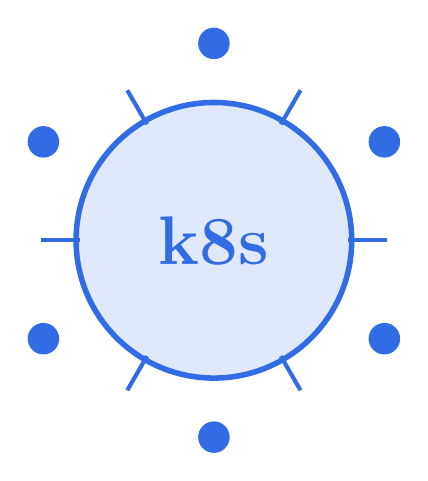
\begin{tikzpicture}
  \node[circle,draw=k8sblue,line width=2pt,minimum size=3.5cm,
        fill=k8sblue!15] (k) {\Huge\color{k8sblue}\textbf{k8s}};
  \foreach \a in {0,60,120,180,240,300}
    \draw[k8sblue,line width=1.5pt] (k.center)+(\a:1.7)--++(\a:2.2);
  \foreach \a in {30,90,150,210,270,330}
    \node[circle,fill=k8sblue,minimum size=0.4cm] at ($(k.center)+(\a:2.5)$) {};
\end{tikzpicture}

\vspace{1.5cm}
{\Large\bfseries N3almou Kubernetes\\
bel projet mte3na ka example pratique}\\[0.5cm]

{\large Vagrant $\cdot$ Ansible $\cdot$ containerd $\cdot$ Flannel $\cdot$ Gitea $\cdot$ Nexus $\cdot$ Jenkins}

\vfill
\begin{minipage}{0.75\textwidth}
\begin{mdframed}[backgroundcolor=k8sblue!10,linecolor=k8sblue,linewidth=0.8pt,
  innerleftmargin=10pt,innerrightmargin=10pt,innertopmargin=8pt,innerbottommargin=8pt]
\centering
\textbf{El hadaf mte3 ktib heda:}\\
Nfehmou Kubernetes b \tuni{3a9l} moch b \tuni{7fadh}.\\
Chaque concept: \emph{chnoua}, \emph{3leh}, \emph{kifeh}, \emph{fel projet mte3na}.
\end{mdframed}
\end{minipage}

\vspace{1cm}
{\small Edition 2026 --- v1.0}
\end{titlepage}

% ---------- TOC ---------------------------------------------------------------
\tableofcontents
\cleardoublepage

% ---------- Preface -----------------------------------------------------------
\chapter*{Mo9addima}
\addcontentsline{toc}{chapter}{Mo9addima}

\tuni{Ya sa7bi}, ken enti ta9ra ktib heda, ya5i 3andek fekra 3la Docker wla 3andek cluster 5edem bel Vagrant ki mte3na, wla ghir 7abb tef7em \tech{Kubernetes}. Kolha behi.

\section*{3leh el ktib heda ma5telef?}

Barcha documentation 3la Kubernetes mawjouda online, ama fi ktib heda:
\begin{itemize}
  \item \textbf{Kol concept} n7akiw 3leh b \tuni{4 questions}: \emph{chnoua}, \emph{3leh mawjoud}, \emph{kifeh y5addem}, \emph{fel projet mte3na kifeh}.
  \item \textbf{El commands} kol wa7ed menhom m3a explication chnoua y3ni.
  \item \textbf{El projet mte3na} (4 VMs: master + 2 workers + services) hiya el \tuni{terrain} bech nfehmou kol 7aja 3la 7ssab.
  \item \textbf{Bel darija}: kelmet arabiya b transliteration (3=ع, 7=ح, 9=ق, 8=غ, 5=خ), kelmet français, w \textbf{el technical terms tob9a b English} kima lezem.
\end{itemize}

\section*{Kifeh ta9ra el ktib heda}

\begin{itemize}
  \item Lou ken enti \textbf{beginner}: 9ra Part 1 b tertib, ma t5alliwch chapter.
  \item Lou ken enti \textbf{3andek ex3érience m3a Docker}: tnajem tebda men Chapter 2 (Core Concepts) w taqfez 3al Architecture.
  \item Lou ken enti \textbf{7abb tawel tefhem el projet mte3na}: Part 2 kolo 3la el tools (Vagrant, Ansible, Gitea, Nexus, Jenkins).
  \item Lou ken enti \textbf{bech ta3mel demo}: rou7 Part 3 Chapter 14 (kubectl mastery) w Chapter 16 (Troubleshooting).
\end{itemize}

\begin{notebox}
\textbf{Rule \#1 fel Kubernetes:} \tuni{Ma te7fedhch, efhem!} \tech{kubectl} 3andha 100+ commands. 7ad ma ya7fedhom kol. El mohim tefhem el model (Pod, Service, Deployment...) w ba3d el documentation \texttt{kubectl --help} tkafi.
\end{notebox}

\cleardoublepage

% =============================================================================
% PART 1: KUBERNETES FUNDAMENTALS
% =============================================================================
\part{Kubernetes Fundamentals --- El Asesiyet}

\chapter{Introduction: Chnoua Kubernetes w 3leh?}

\section{El mochkla: 3leh 5lewna Kubernetes?}

\tuni{Tsawar m3aya hedhi el situation:} 3andek \tuni{micro-service} mektoub bel Node.js, w 7abbit t5addmou 3al production.

\begin{enumerate}
  \item Bedit ya5dem m3a \tech{Docker}: \cmd{docker run my-app}. Behi.
  \item El service wlet 3andou traffic barcha. Lezmek 3 copies (\tuni{n3amlou replicas}).
  \item \tech{Docker Swarm}? Ken mawjoud ama limité. W lou ken VM tmout? El pods ykhosrou.
  \item Kifeh n3amlou \textbf{rolling update} sans downtime?
  \item Kifeh nsit\'e3mlou \textbf{NFS storage} w yochar3ou 3al replicas?
  \item Kifeh n7akou m3a microservices o5rin b \textbf{service discovery}?
\end{enumerate}

Kol ma zedt fel scale, kol ma el mochakel twelli akther. \textbf{Kubernetes} je jébed el solution: platform t\'e5adem kol hedha \tuni{awtomatik}.

\section{Chnoua Kubernetes 9ala dénition}

\begin{conceptbox}[Kubernetes (K8s)]
\textbf{Kubernetes} (isakha 5amm: \tuni{K8s} --- 8 7arf bin K w S) hiya \tuni{container orchestration platform} open-source, 5arjet men Google (Borg project), mawjouda deldhi t7at el \tech{CNCF} (Cloud Native Computing Foundation).

\textbf{El job mte3ha:} ta5dem containers fi cluster mta3 machines, \tuni{tdir 3lihom}, tsay7ihom ki ymoutou, ta3mel scale, networking, storage, kol 7aja.
\end{conceptbox}

\subsection{Kubernetes = System Operating lel Data Center}

\tuni{Tsawar Kubernetes kima Linux ama lel cluster:}
\begin{itemize}
  \item Linux ydir fi \textbf{processes} (fork, schedule, kill) 3la machine we7da.
  \item Kubernetes ydir fi \textbf{pods} (create, schedule, restart) 3la cluster mta3 machines.
\end{itemize}

\section{Container Orchestration: El Mochkla w El 7al}

\subsection{9bal Kubernetes: Era el 3a7di}

9bal Kubernetes (w 9bal Docker 7ata), el applications ka\'inou t5edem 3la \tuni{VM monolithique}. Update = downtime. Scaling = tch\'eri machine jdida.

Ba3d je \tech{Docker} (2013) w rj3et el containers mouch 7aja teoretique. Ama mochkla jdida:
\begin{itemize}
  \item Kifeh n7akou bin 50 container?
  \item Win ne7atouhom (kol container 3la anhi machine)?
  \item Ki ymout container, chkoun y3awdou?
  \item Kifeh n3amlou upgrade sans downtime?
\end{itemize}

\subsection{Solutions historiques: Docker Swarm vs Mesos vs Kubernetes}

\begin{longtable}{L{3.5cm}L{4cm}L{5.5cm}}
\toprule
\textbf{Solution} & \textbf{Mizatha} & \textbf{Mochakelha} \\
\midrule
\tech{Docker Swarm} & B\'essat, integrated m3a Docker & Features limités, community \tuni{matet} \\
\tech{Apache Mesos} & Scale kbir (Twitter, Airbnb) & Complex, learning curve \tuni{qatila} \\
\tech{Nomad} (HashiCorp) & B\'essat, binary we7da & Ecosystem petit compared to K8s \\
\tech{Kubernetes} & Standard industry, ecosystem enorme & Complex lel beginners \\
\bottomrule
\end{longtable}

\subsection{3leh Kubernetes rbe7?}

\begin{enumerate}
  \item \textbf{Backed by Google}: 15+ ans mte3 experience m3a Borg.
  \item \textbf{Open Source + CNCF}: Ma thkomchi charika we7da, governance ouverte.
  \item \textbf{Extensible}: CRDs, Operators, Webhooks --- tnajem tzid 3lih chnoua ma 7abbit.
  \item \textbf{Ecosystem}: Helm, Prometheus, Istio, ArgoCD --- kolhom Kubernetes-native.
  \item \textbf{Cloud Support}: Kol cloud kbir 3andou managed K8s (EKS, GKE, AKS).
\end{enumerate}

\section{Waqtech nest3mlou Kubernetes w waqtech la?}

\begin{tipbox}
\textbf{Kubernetes mouch toujours el solution.} T5edem m\'egha applications moderne scalable. Ama lou ken 3andek \tuni{site statique} wla \tuni{1 container}, Docker wa7dou yekfi.
\end{tipbox}

\subsection{Use cases naj7in (nest3mlou K8s)}

\begin{itemize}
  \item \textbf{Microservices}: Apps fihom 10+ services b languages mo5telfin.
  \item \textbf{High Availability}: Lezem el service mayet9afelch abadan.
  \item \textbf{Auto-scaling}: Traffic yetghayyar (e.g., e-commerce fel soldes).
  \item \textbf{Multi-environment}: Dev, Staging, Prod 3la nafs el infrastructure.
  \item \textbf{CI/CD moderne}: Deploy 3la demande, rollback f\'essa3.
\end{itemize}

\subsection{Use cases khayyeb (MA nest3mlouch K8s)}

\begin{itemize}
  \item \textbf{Monolithic app b 1 service}: Docker Compose yekfi.
  \item \textbf{Team ma ya3rafch DevOps}: K8s complex, ta7 \'ti wa9t 3al learning curve.
  \item \textbf{Budget petit}: Managed K8s (EKS/GKE) y5alef akther mel simple VM.
  \item \textbf{Stateful apps bessif}: Databases fel K8s mumkinet ama mouch \tuni{best practice} toujours.
\end{itemize}

\section{Roadmap mte3 el ktib heda}

Fi \textbf{Part 1}, bech n7akou 3la el fundamentals: Pods, Nodes, Services, Deployments --- el bricks asesiyet. Ba3d n'a9r'ou 3al Architecture (API Server, etcd, Scheduler...). Networking w Storage w Security 7assin lezmet.

Fi \textbf{Part 2}, bech nchouf el tools: Vagrant, Ansible, containerd, Flannel, Gitea, Nexus, Jenkins --- kolhom fel projet mte3na.

Fi \textbf{Part 3}, \tuni{5din 3al pratique}: kubectl mastery, YAML manifests, troubleshooting, production readiness.

Fi \textbf{Part 4}, kifeh tkammel learning --- certifications, resources, next steps.

\cleardoublepage

% =============================================================================
\chapter{Core Concepts --- El Mafehim El Asesiya}

\tuni{Hedha chapter el akher ahammiya.} Lou ken ma tefhemch el concepts heni, kol ba9i el ktib ma yod5olch l'dma8ek. 5din wa9tek.

% ---------- POD ---------------------------------------------------------------
\section{Pod --- El Atom mte3 Kubernetes}

\begin{conceptbox}[Pod]
\textbf{Chnoua:} A9sar 7aja fel Kubernetes. Pod = \tuni{wa7ed wla akther} container, sharing network (IP we7da) w storage (volumes).

\textbf{3leh:} Kubernetes ma y5addemch containers directly, y5addem Pods. \tuni{3leh hakka?} 5atraha applications certaines 7ajetha containers \tuni{toumet} y5admou m3a ba3dhom (sidecar pattern).

\textbf{Fel projet mte3na:} CoreDNS pod, Flannel pod, kube-proxy pod, etcd pod --- kolhom Pods.
\end{conceptbox}

\subsection{Kifeh y5addem Pod?}

\begin{lstlisting}[language=yaml,caption={Pod b\'essat}]
apiVersion: v1
kind: Pod
metadata:
  name: my-nginx
  labels:
    app: nginx
spec:
  containers:
  - name: nginx
    image: nginx:alpine
    ports:
    - containerPort: 80
\end{lstlisting}

\tuni{Commands 3ladaha:}
\begin{lstlisting}
# Ta3mel Pod men YAML
kubectl apply -f my-pod.yaml

# Tchouf el pods mawjoudin
kubectl get pods

# Details mte3 pod
kubectl describe pod my-nginx

# Logs mte3 container fel pod
kubectl logs my-nginx

# D5el 9odhd a pod (kima SSH)
kubectl exec -it my-nginx -- /bin/sh

# Ame7ha
kubectl delete pod my-nginx
\end{lstlisting}

\subsection{Pod Lifecycle}

Pod yedh5al fi phases:
\begin{enumerate}
  \item \tech{Pending}: Ma t5attetch 3la node ba3d (image ma t\'etle3letch, wla ma fama node).
  \item \tech{Running}: Container y5addem.
  \item \tech{Succeeded}: Container kemal, exit 0 (Jobs).
  \item \tech{Failed}: Container tawa exit != 0.
  \item \tech{Unknown}: Kubernetes ma ta3arfch chno\'u y saret (node problem).
\end{enumerate}

\begin{warnbox}
\textbf{Ma ta3melch Pods directly!} 7ta lou ken tnajjem. Pod ki ymout, m\'anouch y3awed. Est3mel \tech{Deployment} bech Kubernetes y3awd\'hom awtomatik.
\end{warnbox}

% ---------- NODE --------------------------------------------------------------
\section{Node --- El Machine (VM wla Physique)}

\begin{conceptbox}[Node]
\textbf{Chnoua:} Machine (VM wla bare-metal) tidor fiha Pods. Node y7ouz \tech{kubelet}, \tech{kube-proxy}, w container runtime.

\textbf{3leh:} El pods lezemhom maken y5admou fih.

\textbf{Fel projet mte3na:} 3 nodes:
\begin{itemize}
  \item \texttt{k8s-master} (192.168.56.10): control plane
  \item \texttt{k8s-worker1} (192.168.56.11): worker
  \item \texttt{k8s-worker2} (192.168.56.12): worker
\end{itemize}
\end{conceptbox}

\subsection{Master vs Worker}

\begin{longtable}{L{3cm}L{6.5cm}L{4cm}}
\toprule
\textbf{Node Type} & \textbf{Components} & \textbf{Y5addem pods user?} \\
\midrule
Master (Control Plane) & API Server, etcd, Scheduler, Controller Manager & \tuni{Par d\'efaut LA} (taint NoSchedule) \\
Worker & kubelet, kube-proxy, containerd & \tuni{AY} (3la daham n7attou apps) \\
\bottomrule
\end{longtable}

\begin{lstlisting}
# Tchouf nodes mawjoudin
kubectl get nodes

# Details kemla
kubectl get nodes -o wide

# Ken node NotReady, 3layh diagnostic
kubectl describe node k8s-worker1

# Cordonh (ma ya7atch 3lih pods jdod)
kubectl cordon k8s-worker1

# Uncordon (ya3aud ya5dem)
kubectl uncordon k8s-worker1

# Drain (ya7aued pods mel node --- mohim 9bal maintenance)
kubectl drain k8s-worker1 --ignore-daemonsets
\end{lstlisting}

% ---------- CLUSTER -----------------------------------------------------------
\section{Cluster --- Majmou3a mta3 Nodes}

\begin{conceptbox}[Cluster]
\textbf{Chnoua:} Majmou3a mta3 Nodes t5addem m3a ba3dhom ka unit we7da, tajm3hom el control plane.

\textbf{3leh:} High availability + scalability. Lou ken node ymout, el pods y3awdou 3la node okhra.

\textbf{Fel projet mte3na:} Cluster b 3 nodes (1 master + 2 workers). \tuni{Single master} (ma7na dev environment, ma3andnach HA).
\end{conceptbox}

% ---------- NAMESPACE ---------------------------------------------------------
\section{Namespace --- T9sim Logique}

\begin{conceptbox}[Namespace]
\textbf{Chnoua:} Namespace = \tuni{folder virtuel} fel cluster. Ya3rez \tuni{ysalik} resources (pods, services, secrets...) lef 3a9la wa7id.

\textbf{3leh:} Bech t9assam el cluster bin teams wla environments (dev, staging, prod) sans cluster jdid.

\textbf{Fel projet mte3na:} \texttt{kube-system} (system pods), \texttt{default} (nos apps), \texttt{kube-flannel} (CNI).
\end{conceptbox}

\subsection{Namespaces b\'ed\'efaut}
\begin{itemize}
  \item \texttt{default}: Resources par d\'efaut.
  \item \texttt{kube-system}: System pods (coredns, kube-proxy...). \tuni{Ma t5assarch fih}.
  \item \texttt{kube-public}: Public, readable mel kol el users.
  \item \texttt{kube-node-lease}: Node heartbeats.
\end{itemize}

\begin{lstlisting}
# List namespaces
kubectl get namespaces

# Resources fi namespace
kubectl get pods -n kube-system

# Kol el namespaces
kubectl get pods -A

# Ta3mel namespace jdid
kubectl create namespace my-app

# Default namespace lel session
kubectl config set-context --current --namespace=my-app
\end{lstlisting}

% ---------- LABELS & SELECTORS ------------------------------------------------
\section{Label \& Selector --- Kifeh Kubernetes Ylawej}

\begin{conceptbox}[Label]
\textbf{Chnoua:} Key-value pair (e.g., \texttt{app=nginx}, \texttt{env=prod}) ta3bet 3la resources.

\textbf{3leh:} Kubernetes ma ye7kemch b names. Ye7kem b \tuni{groupes}. Labels hiya el way to make groups.

\textbf{Kifeh y5addem:} Service, Deployment, w controllers o5rin ylawejhou 3la pods b \textbf{selector}.
\end{conceptbox}

\begin{lstlisting}[language=yaml]
metadata:
  labels:
    app: web
    tier: frontend
    env: production
\end{lstlisting}

\begin{lstlisting}
# Kol pods b label app=nginx
kubectl get pods -l app=nginx

# Multiple labels (AND)
kubectl get pods -l app=nginx,env=prod

# NOT
kubectl get pods -l 'env!=dev'

# Add label 3ad live
kubectl label pod my-nginx version=v1
\end{lstlisting}

% ---------- DEPLOYMENT --------------------------------------------------------
\section{Deployment --- El Manager mte3 Pods}

\begin{conceptbox}[Deployment]
\textbf{Chnoua:} Object y3arref \tuni{chnoua 5erez bech y5addem} (image, replicas, update strategy).

\textbf{3leh:} Pods directly = hasheb. Deployment = decl\'arative --- ent\'ik tgoul "7abb 3 copies mte3 nginx", Kubernetes y5addem bech tkoun \tuni{toujours} 3 copies.

\textbf{Kifeh y5addem:} Deployment y5arez \tech{ReplicaSet}, ReplicaSet y5arez \tech{Pods}. Chaine mta3 ownership.
\end{conceptbox}

\subsection{Example: nginx Deployment}

\begin{lstlisting}[language=yaml,caption={nginx Deployment b 3 replicas}]
apiVersion: apps/v1
kind: Deployment
metadata:
  name: nginx-deployment
spec:
  replicas: 3
  selector:
    matchLabels:
      app: nginx
  template:
    metadata:
      labels:
        app: nginx
    spec:
      containers:
      - name: nginx
        image: nginx:1.25
        ports:
        - containerPort: 80
        resources:
          requests:
            cpu: "100m"
            memory: "128Mi"
          limits:
            cpu: "500m"
            memory: "256Mi"
\end{lstlisting}

\begin{lstlisting}
# Deploy
kubectl apply -f nginx-deployment.yaml

# Scale
kubectl scale deployment nginx-deployment --replicas=5

# Update image (rolling update automatique)
kubectl set image deployment/nginx-deployment nginx=nginx:1.26

# Rollout status
kubectl rollout status deployment/nginx-deployment

# History
kubectl rollout history deployment/nginx-deployment

# Rollback
kubectl rollout undo deployment/nginx-deployment

# Rollback l'n revision specifique
kubectl rollout undo deployment/nginx-deployment --to-revision=2
\end{lstlisting}

% ---------- REPLICASET --------------------------------------------------------
\section{ReplicaSet --- El Garde mte3 Replicas}

\begin{conceptbox}[ReplicaSet]
\textbf{Chnoua:} Controller ydammen n\'omro exact mel pods y5admou toujours.

\textbf{3leh:} Ki ymout pod, ReplicaSet y3awed jdid awtomatik.

\textbf{Fel projet mte3na:} Ma ta3mlouhach directly. \textbf{Deployment} ya5rezhalak.
\end{conceptbox}

% ---------- SERVICE -----------------------------------------------------------
\section{Service --- Networking Stable}

\begin{conceptbox}[Service]
\textbf{Chnoua:} Object ya3tik \tuni{IP permanente} + DNS name lel groupe mte3 Pods.

\textbf{3leh:} Pods IPs yetghayyrou (ki ymout w ya3aud ya5rez, IP jdida). Service ya3tik \tuni{stable endpoint}.

\textbf{Kifeh:} Service ylawej b label selector 3la pods. \tech{kube-proxy} y3amel iptables/ipvs rules.
\end{conceptbox}

\subsection{4 Types mte3 Services}

\begin{longtable}{L{3.5cm}L{4.5cm}L{5.5cm}}
\toprule
\textbf{Type} & \textbf{Scope} & \textbf{Use Case} \\
\midrule
\tech{ClusterIP} (default) & Internal only & Microservice-to-microservice \\
\tech{NodePort} & External (port 30000-32767 3la kol node) & Dev, testing, simple external \\
\tech{LoadBalancer} & External (cloud LB) & Production 3al cloud \\
\tech{ExternalName} & DNS CNAME & Alias l\'service 5arej el cluster \\
\bottomrule
\end{longtable}

\begin{lstlisting}[language=yaml,caption={Service ClusterIP}]
apiVersion: v1
kind: Service
metadata:
  name: nginx-service
spec:
  type: ClusterIP
  selector:
    app: nginx     # Ylawej 3la pods b label app=nginx
  ports:
  - port: 80       # Port mte3 service
    targetPort: 80 # Port mte3 pod
    protocol: TCP
\end{lstlisting}

\begin{lstlisting}[language=yaml,caption={Service NodePort (external)}]
apiVersion: v1
kind: Service
metadata:
  name: nginx-nodeport
spec:
  type: NodePort
  selector:
    app: nginx
  ports:
  - port: 80
    targetPort: 80
    nodePort: 30080   # M\'etiid entre 30000-32767
\end{lstlisting}

\begin{lstlisting}
# Access: http://<any-node-ip>:30080
curl http://192.168.56.10:30080
curl http://192.168.56.11:30080  # Ay node y5addem!
\end{lstlisting}

% ---------- INGRESS -----------------------------------------------------------
\section{Ingress --- HTTP Routing}

\begin{conceptbox}[Ingress]
\textbf{Chnoua:} Routing rules HTTP/HTTPS mel 5arej lel services.

\textbf{3leh:} NodePort w LoadBalancer service per service = cher. Ingress = \tuni{reverse proxy} (nginx, traefik) y7ouz rules lel kol el apps.

\textbf{Lezem:} Ingress Controller (nginx-ingress, traefik) m\'ectab fel cluster.
\end{conceptbox}

\begin{lstlisting}[language=yaml]
apiVersion: networking.k8s.io/v1
kind: Ingress
metadata:
  name: my-ingress
spec:
  rules:
  - host: app.example.com
    http:
      paths:
      - path: /api
        pathType: Prefix
        backend:
          service:
            name: api-service
            port:
              number: 80
      - path: /
        pathType: Prefix
        backend:
          service:
            name: frontend-service
            port:
              number: 80
\end{lstlisting}

% ---------- CONFIGMAP & SECRET ------------------------------------------------
\section{ConfigMap \& Secret --- Configuration}

\begin{conceptbox}[ConfigMap]
\textbf{Chnoua:} Key-value storage lel \tuni{config data mouch sensitive} (URLs, feature flags, ports...).

\textbf{3leh:} Ma th\'attchi config hard-coded fel image. Separation of concerns.
\end{conceptbox}

\begin{conceptbox}[Secret]
\textbf{Chnoua:} Kima ConfigMap ama lel \tuni{data sensitive} (passwords, tokens, certs). Base64 encoded (\textbf{mouch encrypted by default!}).

\textbf{3leh:} Separation + moins de risque 7tta lou tchouf manifest fel git.
\end{conceptbox}

\begin{lstlisting}[language=yaml]
# ConfigMap
apiVersion: v1
kind: ConfigMap
metadata:
  name: app-config
data:
  database_url: "postgres://db:5432/mydb"
  log_level: "INFO"
---
# Secret
apiVersion: v1
kind: Secret
metadata:
  name: db-secret
type: Opaque
data:
  password: cGFzc3dvcmQxMjM=  # base64: password123
\end{lstlisting}

\begin{lstlisting}[language=yaml,caption={Injection fel Pod}]
spec:
  containers:
  - name: app
    image: myapp:v1
    env:
    - name: DATABASE_URL
      valueFrom:
        configMapKeyRef:
          name: app-config
          key: database_url
    - name: DB_PASSWORD
      valueFrom:
        secretKeyRef:
          name: db-secret
          key: password
\end{lstlisting}

\begin{warnbox}
\textbf{Secret b base64 mouch s\'ecurity!} \texttt{echo cGFzc3dvcmQ= | base64 -d} = \texttt{password}. Enable \tuni{encryption at rest} fel etcd, wla est3mel Vault / Sealed Secrets lel production.
\end{warnbox}

% ---------- VOLUMES -----------------------------------------------------------
\section{Volume \& PersistentVolume --- Storage}

\begin{conceptbox}[Volume]
\textbf{Chnoua:} Directory m3a data, mounted fel container.

\textbf{3leh:} Container filesystem \tuni{ephemeral} --- ki container ymout, data t\'edhra3. Volume \'etd\'aom.
\end{conceptbox}

\subsection{Volume Types}

\begin{longtable}{L{3cm}L{7cm}L{3.5cm}}
\toprule
\textbf{Type} & \textbf{Description} & \textbf{Lifetime} \\
\midrule
\texttt{emptyDir} & Directory empty created ki pod yabda & Pod lifetime \\
\texttt{hostPath} & Directory mel node filesystem & Node lifetime \\
\texttt{configMap} & Mount ConfigMap as files & --- \\
\texttt{secret} & Mount Secret as files & --- \\
\texttt{nfs} & NFS share (\emph{fel projet mte3na!}) & Permanent \\
\texttt{persistentVolumeClaim} & Claim 3la PV dynamique & Permanent \\
\bottomrule
\end{longtable}

\begin{conceptbox}[PersistentVolume (PV) + PersistentVolumeClaim (PVC)]
\textbf{PV:} Storage resource fel cluster (like a "disk"). Admin y5al9ou.

\textbf{PVC:} Request mel user: "7abb 5 GB storage ReadWriteOnce". Kubernetes ylawej 3la PV m\'etlaim.

\textbf{Fel projet mte3na:} NFS server 3al services VM. Tnajem ta3mel PV y\'pointer 3la \texttt{192.168.56.20:/srv/nfs/mysql-data}.
\end{conceptbox}

\begin{lstlisting}[language=yaml,caption={PV + PVC m3a NFS}]
apiVersion: v1
kind: PersistentVolume
metadata:
  name: nfs-pv
spec:
  capacity:
    storage: 5Gi
  accessModes:
    - ReadWriteMany
  nfs:
    server: 192.168.56.20
    path: /srv/nfs/mysql-data
---
apiVersion: v1
kind: PersistentVolumeClaim
metadata:
  name: nfs-pvc
spec:
  accessModes:
    - ReadWriteMany
  resources:
    requests:
      storage: 5Gi
\end{lstlisting}

% ---------- DAEMONSET ---------------------------------------------------------
\section{DaemonSet --- Pod 3la Kol Node}

\begin{conceptbox}[DaemonSet]
\textbf{Chnoua:} Controller ydaman pod we7ed y5addem 3la kol node fel cluster.

\textbf{3leh:} Services n\'odhbethom fi kol machine: logging agent, monitoring agent, CNI plugin...

\textbf{Fel projet mte3na:}
\begin{itemize}
  \item \tech{kube-flannel-ds}: Flannel CNI 3la kol node
  \item \tech{kube-proxy}: 3la kol node
\end{itemize}
\end{conceptbox}

\begin{lstlisting}
# Chouf les DaemonSets
kubectl get daemonsets -A
\end{lstlisting}

% ---------- STATEFULSET -------------------------------------------------------
\section{StatefulSet --- lel Databases}

\begin{conceptbox}[StatefulSet]
\textbf{Chnoua:} Kima Deployment ama lel applications \tuni{stateful} (7aajithom identity fixe, storage fixe, order fixe).

\textbf{3leh:} Databases: MySQL, PostgreSQL, MongoDB, Cassandra, Kafka --- ma tnajjemch t3amelhom Deployment.

\textbf{Features:}
\begin{itemize}
  \item Pods 3andhom names stables (\texttt{mysql-0}, \texttt{mysql-1}, \texttt{mysql-2}).
  \item Storage persistant per pod.
  \item Order mte3 startup/shutdown.
\end{itemize}
\end{conceptbox}

% ---------- JOB & CRONJOB -----------------------------------------------------
\section{Job \& CronJob --- Tasks One-shot}

\begin{conceptbox}[Job]
\textbf{Chnoua:} Run pod wa7ed wla akther l'n job ikmel (e.g., database migration, backup).

\textbf{3leh:} Deployment y5addem toujours. Job y5aden \tuni{marra}, ba3d y9aff.
\end{conceptbox}

\begin{conceptbox}[CronJob]
\textbf{Chnoua:} Job y5adem 3la schedule (cron syntax).

\textbf{3leh:} Tasks dawriya: backup kol y\'oum, cleanup kol sm\'ana...
\end{conceptbox}

\begin{lstlisting}[language=yaml]
apiVersion: batch/v1
kind: CronJob
metadata:
  name: backup-job
spec:
  schedule: "0 2 * * *"   # Kol y\'oum el 2h
  jobTemplate:
    spec:
      template:
        spec:
          containers:
          - name: backup
            image: backup-tool:v1
            command: ["/backup.sh"]
          restartPolicy: OnFailure
\end{lstlisting}

\cleardoublepage

% =============================================================================
\chapter{Architecture --- El Mo5 w El 3odhlat}

Fi chapter heda bech nefhmou \tuni{chnoua mawjoud} gu\'edh chaque node, w kifeh el cluster y5addem mel dekhel.

\section{Control Plane --- El Mo5}

El Control Plane = el components y5admou 3la master node. Howa el \textbf{brain} mte3 el cluster.

\subsection{Architecture Overview}

\begin{center}
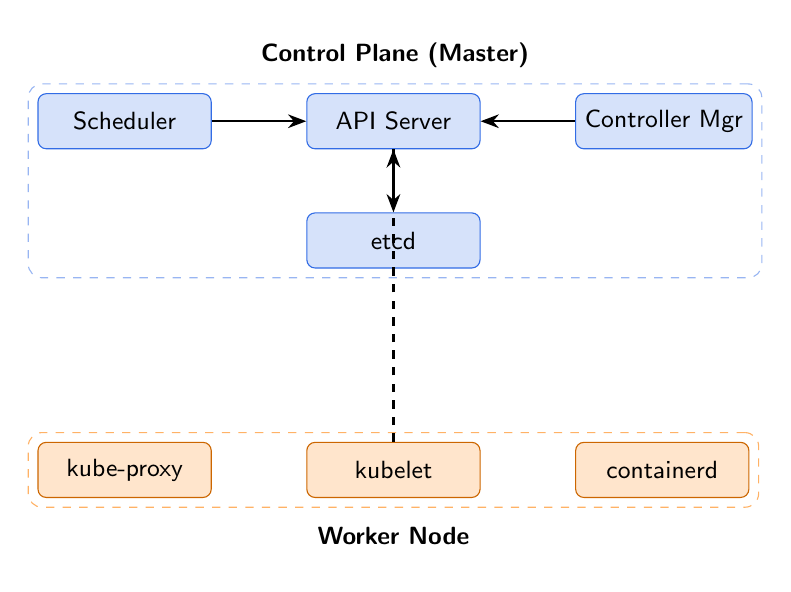
\begin{tikzpicture}[
  node distance=0.8cm and 1.2cm,
  every node/.style={rectangle,draw,rounded corners=3pt,minimum width=2.2cm,minimum height=0.7cm,font=\small\sffamily},
  cp/.style={fill=k8sblue!20,draw=k8sblue},
  worker/.style={fill=orange!20,draw=orange!80!black},
  arr/.style={->,>=Stealth,thick},
]

% Control plane
\node[cp] (api) {API Server};
\node[cp,below=of api] (etcd) {etcd};
\node[cp,left=of api] (sched) {Scheduler};
\node[cp,right=of api] (ctrl) {Controller Mgr};

\node[draw=k8sblue!50,dashed,rounded corners=5pt,
  fit=(sched)(api)(ctrl)(etcd),
  label=above:\textbf{Control Plane (Master)}] {};

% Workers
\node[worker,below=2.2cm of etcd] (kubelet1) {kubelet};
\node[worker,left=of kubelet1] (kproxy1) {kube-proxy};
\node[worker,right=of kubelet1] (cri1) {containerd};

\node[draw=orange!60,dashed,rounded corners=5pt,
  fit=(kproxy1)(kubelet1)(cri1),
  label=below:\textbf{Worker Node}] {};

% Arrows
\draw[arr] (sched) -- (api);
\draw[arr] (ctrl) -- (api);
\draw[arr] (api) -- (etcd);
\draw[arr,dashed] (kubelet1) -- (api);
\end{tikzpicture}
\end{center}

% ---------- API SERVER --------------------------------------------------------
\subsection{API Server --- El B\'ab El Wa7id}

\begin{conceptbox}[kube-apiserver]
\textbf{Chnoua:} REST API (HTTP/HTTPS) howa el seul entry point lel cluster. Kol 7aja \tuni{d\'oukhoulha} w \tuni{5roujha} tadi mennou.

\textbf{3leh:} Centralization = security, audit, validation fi makenet wa7da.

\textbf{Fel projet mte3na:} \texttt{https://192.168.56.10:6443}
\end{conceptbox}

\textbf{Chkoun y\'7ki m3a API Server:}
\begin{itemize}
  \item \texttt{kubectl} (user): HTTPS + kubeconfig file.
  \item \texttt{kubelet} (kol node): HTTPS + client cert.
  \item \texttt{kube-scheduler}, \texttt{kube-controller-manager}: loopback.
  \item \tuni{Chaque pod} ken 7abb y\'7ki m3a K8s API: ServiceAccount token.
\end{itemize}

\begin{lstlisting}
# Tchouf URL mte3 API server
kubectl cluster-info

# Raw API call
kubectl get --raw /api/v1/namespaces/default/pods

# curl direct (b token)
TOKEN=$(kubectl -n default create token default)
curl -k -H "Authorization: Bearer $TOKEN" \
  https://192.168.56.10:6443/api/v1/pods
\end{lstlisting}

% ---------- ETCD --------------------------------------------------------------
\subsection{etcd --- El Memory mte3 El Cluster}

\begin{conceptbox}[etcd]
\textbf{Chnoua:} Distributed key-value store, b\'esd consistent (Raft consensus). Tous les \tuni{state} mte3 el cluster fih.

\textbf{3leh:} Kubernetes stateless --- ki ymout api-server, t\'a5dach. Ama ki ymout etcd, \tuni{kollou khsir}.

\textbf{Chi y\'etsajel fih:} kol object (Pods, Services, ConfigMaps, Secrets, Nodes...) --- every single YAML manifest.
\end{conceptbox}

\begin{warnbox}
\textbf{etcd backup = \tuni{a9sar priority} fi production!} Lou ken etcd cluster y5sar, ma tnajemch t3awed el cluster (unless 3andek backup). Schedule snapshots kol y\'oum.
\end{warnbox}

\begin{lstlisting}
# Snapshot mte3 etcd (3al master)
sudo ETCDCTL_API=3 etcdctl \
  --endpoints=https://127.0.0.1:2379 \
  --cacert=/etc/kubernetes/pki/etcd/ca.crt \
  --cert=/etc/kubernetes/pki/etcd/server.crt \
  --key=/etc/kubernetes/pki/etcd/server.key \
  snapshot save /backup/etcd-$(date +%F).db
\end{lstlisting}

% ---------- SCHEDULER ---------------------------------------------------------
\subsection{Scheduler --- Chkoun Ya5tar El Node}

\begin{conceptbox}[kube-scheduler]
\textbf{Chnoua:} Ki pod jadid mawjoud (pending, ma3andouch node), scheduler y\'a5tar \tuni{anhi node} el monaseb.

\textbf{Algorithm b simplification:}
\begin{enumerate}
  \item \textbf{Filtering}: Anhi nodes mumkinin? (CPU k\'efi, RAM k\'efi, taints compatible, nodeSelector)
  \item \textbf{Scoring}: Anhi a7san? (node a9al loaded, affinity...)
\end{enumerate}
\end{conceptbox}

\textbf{Factors fel scheduling:}
\begin{itemize}
  \item \textbf{Resource requests} (CPU, memory): Node lezem yekkafi.
  \item \textbf{Node Selector}: \texttt{disk: ssd} --- yet5ayyr ghir nodes 3andhom label heda.
  \item \textbf{Affinity / Anti-affinity}: \tuni{attire} wla \tuni{ab3eid} 3la pods.
  \item \textbf{Taints / Tolerations}: Node y\'gou\'l "nombre limit\'e", pod lezmou tol\'eration.
\end{itemize}

% ---------- CONTROLLER MANAGER ------------------------------------------------
\subsection{Controller Manager --- El 7ares}

\begin{conceptbox}[kube-controller-manager]
\textbf{Chnoua:} Process y7ouz kol el controllers. Controller = loop y\'gar\'n \tuni{desired state} vs \tuni{actual state}, w y\'syil differences.

\textbf{Types mte3 controllers:}
\begin{itemize}
  \item \textbf{Deployment Controller}: Ydamen replicas voulus.
  \item \textbf{ReplicaSet Controller}: Ydamen pods comptés.
  \item \textbf{Node Controller}: Ych\'ouf nodes, ymarkehom NotReady ken ma yrespondouch.
  \item \textbf{Job Controller}: Y5arez pods lel jobs.
  \item \textbf{Service Account Controller}: Y5arez default service accounts.
  \item ...w 30+ o5rin.
\end{itemize}
\end{conceptbox}

\subsection{Cloud Controller Manager}

Ken fel cloud (AWS, GCP, Azure), hedha el component y5addem m3a provider: provision LoadBalancers, attach volumes, manage nodes. Fel projet mte3na (Vagrant): \tuni{ma mawjoudch}.

\section{Worker Node Components --- El 3odhlat}

% ---------- KUBELET -----------------------------------------------------------
\subsection{kubelet --- El Agent}

\begin{conceptbox}[kubelet]
\textbf{Chnoua:} Agent y5addem 3la kol node. Y\'7ki m3a API server, ya5ou instructions, w y5adem pods via \tuni{container runtime}.

\textbf{Job mte3ou:}
\begin{enumerate}
  \item Register el node m3a API server.
  \item Watch pods m\'etlas lu node heda.
  \item Start/stop containers via CRI.
  \item Report status (health checks, resource usage) l\'API.
\end{enumerate}

\textbf{Fel projet mte3na:} Config fi \texttt{/etc/kubernetes/kubelet.conf} + \texttt{/etc/default/kubelet}.
\end{conceptbox}

\begin{lstlisting}
# Logs mte3 kubelet (linux systemd)
sudo journalctl -u kubelet -f

# Status
sudo systemctl status kubelet

# Restart (ken mochkla)
sudo systemctl restart kubelet
\end{lstlisting}

% ---------- KUBE-PROXY --------------------------------------------------------
\subsection{kube-proxy --- Network Magic}

\begin{conceptbox}[kube-proxy]
\textbf{Chnoua:} DaemonSet y5addem 3la kol node. Y\'n\'odhem networking rules (iptables wla ipvs) bech Services yemchiwu.

\textbf{Kifeh y5addem:} Ki ta3mel Service, kube-proxy y\'5atet iptables rules:
\begin{itemize}
  \item Traffic l\'ClusterIP \texttt{10.96.0.5} → forward l\'pod IP \texttt{10.244.1.23:80}.
  \item Load balancing (round-robin) bin el pods.
\end{itemize}
\end{conceptbox}

\begin{warnbox}
\textbf{Fel projet mte3na \tuni{sar mochkla kbira}:} kubeadm y5leq kube-proxy kubeconfig m3a IP mel \emph{default-route interface} (NAT: 10.0.2.15), mouch \texttt{--apiserver-advertise-address} (192.168.56.10). Resultat: kube-proxy ma ynajjemch y7ki m3a API, Flannel y\'cracsh\'e, workers NotReady. Fix: patch el ConfigMap. \tuni{Codified fel role master/tasks/main.yml}.
\end{warnbox}

% ---------- CONTAINER RUNTIME -------------------------------------------------
\subsection{Container Runtime --- containerd (moch Docker!)}

\begin{conceptbox}[containerd]
\textbf{Chnoua:} Container runtime --- software y5addem containers directly.

\textbf{3leh moch Docker:}
\begin{itemize}
  \item Docker 3andou CLI + daemon + build --- kbir.
  \item Kubernetes 7ajetou b GH runtime. Docker kan y\'est5dem \texttt{dockershim} (shim) bin kubelet w Docker.
  \item Depuis Kubernetes \textbf{1.24}, \texttt{dockershim} \tuni{enleve}. Containerd (wla CRI-O) asma mou ba\'r\'aha.
  \item Docker images = containerd images (OCI format), \tuni{compatibles}.
\end{itemize}

\textbf{Fel projet mte3na:}
\begin{itemize}
  \item \texttt{SystemdCgroup = true} fel \texttt{/etc/containerd/config.toml}.
  \item \texttt{sandbox\_image = "registry.k8s.io/pause:3.9"}.
\end{itemize}
\end{conceptbox}

\begin{conceptbox}[CRI --- Container Runtime Interface]
\textbf{Chnoua:} API standard bin kubelet w container runtime.

\textbf{3leh:} Kubernetes ma 7abbchi y\'atblej m3a runtime we7ed. CRI = plugin interface. Ay runtime mo7taram CRI (containerd, CRI-O) ymkin\'i y5addem m3a K8s.
\end{conceptbox}

\begin{lstlisting}
# Crictl --- CLI like docker ama lel CRI
sudo crictl ps          # Containers working
sudo crictl images      # Images
sudo crictl logs <id>   # Logs
\end{lstlisting}

\section{Add-ons --- El Plugins}

\subsection{CNI --- Container Network Interface}

\begin{conceptbox}[CNI]
\textbf{Chnoua:} Standard + plugins bech pods y7aki b\'enaat hom + m3a 5arej.

\textbf{3leh:} Kubernetes ma y\'hach networking implementation. T5ayer CNI plugin 3la 7sab needs.

\textbf{Fel projet mte3na:} \tech{Flannel} (VXLAN overlay, b\'essat). Alternatives: Calico (BGP + policies), Cilium (eBPF, advanced).
\end{conceptbox}

\subsection{CoreDNS --- Service Discovery}

\begin{conceptbox}[CoreDNS]
\textbf{Chnoua:} DNS server y5addem fi pods fel cluster.

\textbf{3leh:} Pods y3arfou y7akou m3a services b names: \texttt{my-service.default.svc.cluster.local} au lieu de IP.

\textbf{Fel projet mte3na:} 2 pods \texttt{coredns-*} fi kube-system namespace.
\end{conceptbox}

\subsection{Metrics Server --- Ressources}

\begin{conceptbox}[Metrics Server]
\textbf{Chnoua:} Collect CPU/memory usage pour pods w nodes.

\textbf{3leh:} \texttt{kubectl top} ma t5addemch bidoun. Lezmou lel HPA (autoscaling).

\textbf{Fel projet mte3na:} \tuni{Ma m\'ectabch}. Ken 7abbit t\'est5dem \cmd{kubectl top nodes}, lezem t\'installer metrics-server.
\end{conceptbox}

\cleardoublepage

% =============================================================================
\chapter{Networking --- El Chabka}

\tuni{Heda el chapter el akher critique.} Networking fel K8s s3ib \'awal marra, ama ki tefhmou, el kol yewdh7.

\section{Network Model mte3 Kubernetes}

\subsection{4 r\'egles asesiyet}

Kubernetes y\'farar chroo7 network b regles \tuni{net}:
\begin{enumerate}
  \item \textbf{Pod-to-Pod}: Kol pod 3andou IP unique. Pods y7akou directly, \tuni{sans NAT}, mel ay node.
  \item \textbf{Pod-to-Service}: Via ClusterIP (virtual). kube-proxy ydir DNAT.
  \item \textbf{External-to-Service}: Via NodePort, LoadBalancer, Ingress.
  \item \textbf{Network Policies}: Firewall rules bin pods (defense-in-depth).
\end{enumerate}

\subsection{Flat Network Model}

\begin{tipbox}
\textbf{El diff\'erence el kbira vs Docker classique:} Docker ta3mel NAT + port mapping. K8s LA. Kol pod 3andou \tuni{IP vraie} fel network 3am mte3 el cluster. T7aki m3a pod 3la node o5ra = kima t7aki m3a pod 3la nafs node.
\end{tipbox}

\section{IP Ranges fel Projet Mte3na}

\begin{center}
\begin{tabular}{lll}
\toprule
\textbf{Network} & \textbf{CIDR} & \textbf{Usage} \\
\midrule
VM Network (host-only) & \texttt{192.168.56.0/24} & VMs inter-communication \\
Pod Network (Flannel) & \texttt{10.244.0.0/16} & Pod IPs (overlay) \\
Service Network & \texttt{10.96.0.0/12} & ClusterIP virtual IPs \\
\bottomrule
\end{tabular}
\end{center}

\textbf{Chnoua ya3ni hedha pratiquement:}
\begin{itemize}
  \item Node IPs: \texttt{192.168.56.10, .11, .12, .20}
  \item Pods 3la worker1 mumkin yekhdhou: \texttt{10.244.1.2, 10.244.1.3...}
  \item Pods 3la worker2: \texttt{10.244.2.2, 10.244.2.3...}
  \item Services: \texttt{10.96.0.1} (kubernetes API service), \texttt{10.96.0.10} (coredns)...
\end{itemize}

\section{CNI Deep Dive: Flannel}

\subsection{VXLAN Encapsulation}

Flannel y5addem b \textbf{VXLAN}: overlay network fouq UDP.

\begin{itemize}
  \item Pod 3la worker1 (\texttt{10.244.1.5}) 7abb y\'rasel pod 3la worker2 (\texttt{10.244.2.8}).
  \item Packet yet\'7att fi UDP packet jdid (encapsulation), yem'si men \texttt{192.168.56.11} l'\texttt{192.168.56.12}.
  \item Flannel 3al worker2 y\'d\'ecapsulate, y\'rassel lel pod cible.
\end{itemize}

\begin{warnbox}
\textbf{Mochkla fel dual-NIC (fel projet mte3na):} VMs 3andhom 2 NICs: \texttt{enp0s3} (NAT) w \texttt{enp0s8} (host-only). Flannel default y\'5atar enp0s3, ma 7akchi m3a nodes o5rin. \tuni{Fix:} \texttt{--iface=enp0s8} fel Flannel manifest (fel role \texttt{cni}).
\end{warnbox}

\subsection{Alternatives lel Flannel}

\begin{longtable}{L{2.5cm}L{5cm}L{5.5cm}}
\toprule
\textbf{CNI} & \textbf{Strengths} & \textbf{Weaknesses} \\
\midrule
Flannel & B\'essat, stable, 5atr learn & Ma fihoulsh Network Policies \\
Calico & Policies, BGP (mouch overlay), fast & Config plus complex \\
Cilium & eBPF, observability, policies L7 & Kernel 4.9+, courbe d'apprentissage \\
Weave & P2P mesh, easy & Performance moins bonne \\
\bottomrule
\end{longtable}

\section{Service Discovery --- DNS}

Kol namespace 3andou DNS sous-d\'omaine. Format:
\begin{center}
\texttt{<service>.<namespace>.svc.cluster.local}
\end{center}

\textbf{Examples:}
\begin{itemize}
  \item \texttt{kubernetes.default.svc.cluster.local} → API server (10.96.0.1)
  \item \texttt{my-app.default.svc.cluster.local} → Service \texttt{my-app} fi default namespace
  \item Mel pod same namespace: \texttt{my-app} yekfi (short name)
\end{itemize}

\begin{lstlisting}
# T5oud DNS mel pod
kubectl run -it --rm debug --image=busybox --restart=Never -- sh
/ # nslookup kubernetes
Server:    10.96.0.10
Address 1: 10.96.0.10 kube-dns.kube-system.svc.cluster.local

Name:      kubernetes
Address 1: 10.96.0.1 kubernetes.default.svc.cluster.local
\end{lstlisting}

\section{Network Policies --- Firewall lel Pods}

\begin{conceptbox}[NetworkPolicy]
\textbf{Chnoua:} Rules bech t5tar \tuni{anhi pod ynajjem yaqra l'anhi pod}.

\textbf{3leh:} Defense-in-depth. Microsegmentation. Zero Trust.

\textbf{Lezem:} CNI m\'estajib (Calico, Cilium, Weave). \tuni{Flannel MA IMPLEMENTCH NetworkPolicies!}
\end{conceptbox}

\begin{lstlisting}[language=yaml,caption={Deny-all ingress par d\'efault}]
apiVersion: networking.k8s.io/v1
kind: NetworkPolicy
metadata:
  name: default-deny-ingress
  namespace: default
spec:
  podSelector: {}
  policyTypes:
  - Ingress
\end{lstlisting}

\cleardoublepage

% =============================================================================
\chapter{Storage --- El Stockage}

\section{El mochkla: Containers Ephemeral}

Container filesystem \tuni{ya5sar} ki container ymout. Lou ken 3andek database, logs, uploads... kollou yroh.

\textbf{Solution:} Volumes.

\section{Volume Types Par D\'efault}

\subsection{emptyDir --- Temporaire}

\begin{lstlisting}[language=yaml]
spec:
  containers:
  - name: app
    volumeMounts:
    - mountPath: /cache
      name: cache-vol
  volumes:
  - name: cache-vol
    emptyDir: {}
\end{lstlisting}
\textbf{Lifetime:} Pod lifetime. Ki pod ymout, data y\'en\'jr\'af.

\subsection{hostPath --- Node Filesystem}

\begin{lstlisting}[language=yaml]
volumes:
- name: data
  hostPath:
    path: /var/data
    type: DirectoryOrCreate
\end{lstlisting}

\begin{warnbox}
\textbf{hostPath \tuni{dangerous}!} Pod yqra/yakteb fi filesystem mte3 el node --- security risk. Data tied l\'node --- ki pod yetnaql, data ma yefotch m3ah. \tuni{Ma t\'est5dmoch} sauf lel system pods.
\end{warnbox}

\subsection{NFS --- Network Shared Storage}

\begin{lstlisting}[language=yaml]
volumes:
- name: mysql-data
  nfs:
    server: 192.168.56.20
    path: /srv/nfs/mysql-data
\end{lstlisting}

\begin{tipbox}
\textbf{Fel projet mte3na:} NFS server 3al services VM. Kol el nodes ynajmou mount \texttt{/srv/nfs/mysql-data}. \tuni{Perfect} lel \texttt{ReadWriteMany} use cases (multiple pods y\'9rawa w yketbou m3a ba3dhom).
\end{tipbox}

\section{PersistentVolume \& PersistentVolumeClaim}

\subsection{El Pattern}

\begin{enumerate}
  \item \textbf{Admin}: Y5arez PVs (wla StorageClass pour dynamic provisioning).
  \item \textbf{User}: Y5arez PVC (request: "7abb 5Gi, ReadWriteOnce").
  \item \textbf{Kubernetes}: Y\'bind PVC m3a PV moul9em.
  \item \textbf{Pod}: Y\'mount el PVC.
\end{enumerate}

\subsection{Access Modes}

\begin{itemize}
  \item \texttt{ReadWriteOnce (RWO)}: Un seul node ynajm y\'write.
  \item \texttt{ReadOnlyMany (ROX)}: Multiple nodes read-only.
  \item \texttt{ReadWriteMany (RWX)}: Multiple nodes read-write (NFS supports heda).
\end{itemize}

\subsection{StorageClass --- Dynamic Provisioning}

\begin{conceptbox}[StorageClass]
\textbf{Chnoua:} T\'odhbet \tuni{kifeh} yet5al9ou PVs awtomatik.

\textbf{3leh:} Admin ma y3amelch PVs manually. StorageClass + PVC = PV jdid awtomatik.

\textbf{Examples:} \texttt{aws-ebs-gp3}, \texttt{gce-pd-ssd}, \texttt{local-path} (dev), \texttt{nfs-provisioner}.
\end{conceptbox}

\cleardoublepage

% =============================================================================
\chapter{Security --- El Sécurité}

\section{Authentication \& Authorization}

\subsection{Chkoun t\'a5atab m3a API?}

\textbf{3 questions lezem API Server yjawab 3lihom:}
\begin{enumerate}
  \item \textbf{Authentication}: \tuni{Chkoun enta?} (certificates, tokens, OIDC)
  \item \textbf{Authorization}: \tuni{Chnoua 7a9ek ta3mel?} (RBAC, ABAC, Webhook)
  \item \textbf{Admission Control}: \tuni{Request mte3ak valide?} (mutation + validation)
\end{enumerate}

\subsection{ServiceAccount --- Identity lel Pods}

\begin{conceptbox}[ServiceAccount]
\textbf{Chnoua:} Account \tuni{non-human} y\'est5d\'moulha les pods l\'yet7akou m3a API server.

\textbf{3leh:} Chaque pod yelzmou identity lou yeqra secrets wla y3amel actions fel cluster.

\textbf{Par d\'efault:} Kol namespace fih \texttt{default} ServiceAccount. Pod y5odhha ken ma t\'od\'bt\'sh wa7ed o5ra.
\end{conceptbox}

\subsection{RBAC --- Role-Based Access Control}

\begin{conceptbox}[RBAC]
\textbf{4 concepts:}
\begin{itemize}
  \item \texttt{Role}: Permissions fi namespace specifique.
  \item \texttt{ClusterRole}: Permissions 3la kol el cluster.
  \item \texttt{RoleBinding}: Rabt Role m3a User/Group/SA fi namespace.
  \item \texttt{ClusterRoleBinding}: Rabt cluster-wide.
\end{itemize}
\end{conceptbox}

\begin{lstlisting}[language=yaml,caption={Read-only Role lel pods}]
apiVersion: rbac.authorization.k8s.io/v1
kind: Role
metadata:
  name: pod-reader
  namespace: default
rules:
- apiGroups: [""]
  resources: ["pods"]
  verbs: ["get", "list", "watch"]
---
apiVersion: rbac.authorization.k8s.io/v1
kind: RoleBinding
metadata:
  name: bind-pod-reader
  namespace: default
subjects:
- kind: ServiceAccount
  name: my-sa
  namespace: default
roleRef:
  kind: Role
  name: pod-reader
  apiGroup: rbac.authorization.k8s.io
\end{lstlisting}

\section{Secrets Management}

\begin{warnbox}
\textbf{Secrets fel K8s b base64 \tuni{mouch} encrypted par d\'efault!} \tuni{Lezem} t\'enable \tuni{encryption at rest} fel etcd, wla t\'est5dem solutions o5rin.
\end{warnbox}

\subsection{Solutions pour Secrets}

\begin{itemize}
  \item \textbf{etcd encryption at rest}: Minimum hygiene.
  \item \textbf{HashiCorp Vault}: Gold standard. Dynamic secrets, audit, rotation.
  \item \textbf{Sealed Secrets} (Bitnami): Encrypt secrets fel Git (GitOps-friendly).
  \item \textbf{External Secrets Operator}: Sync secrets men Vault/AWS SM/GCP SM.
\end{itemize}

\section{Pod Security Standards}

3 profiles officiels (remplacent PodSecurityPolicies dh\'r\'eou):

\begin{longtable}{L{3cm}L{8cm}}
\toprule
\textbf{Profile} & \textbf{Description} \\
\midrule
\texttt{Privileged} & Kol 7aja mumkin. \tuni{Ma t\'est5dmoch fel prod}. \\
\texttt{Baseline} & Restrictions minimales (no privileged containers, no host namespaces). \\
\texttt{Restricted} & Highly restricted (non-root, read-only fs, no capabilities). \\
\bottomrule
\end{longtable}

\section{Network Security}

D\'ej\'a vu: NetworkPolicies (chapter 4). \textbf{Rules:}
\begin{itemize}
  \item Default deny all.
  \item Explicit allow per namespace/service.
  \item Ingress + egress controls.
\end{itemize}

\cleardoublepage

% =============================================================================
\chapter{Workload Management}

\section{Deployment Strategies}

\subsection{Rolling Update (default)}

\begin{conceptbox}[Rolling Update]
Kubernetes y\'replaces pods \tuni{t\'edr\'ija} --- ya5erz pod jdid, ya7aut a9odaim ba3d test.

\textbf{Zero downtime} ken configuré b readiness probes + maxUnavailable + maxSurge.
\end{conceptbox}

\begin{lstlisting}[language=yaml]
spec:
  strategy:
    type: RollingUpdate
    rollingUpdate:
      maxUnavailable: 1   # 1 pod out 3al ma5oud
      maxSurge: 1         # 1 pod extra allowed during update
\end{lstlisting}

\subsection{Recreate}

Kill kol el pods, ba3d y5arez new. \textbf{Downtime mawjoud}. Use case: apps qui ne peuvent pas coexist v1 + v2.

\subsection{Blue/Green}

Deux environnements complets (blue = current, green = new). Switch traffic b service selector. \tuni{Ma t\'intnach mech native}, tnajem ta3mlou m3a labels.

\subsection{Canary}

Deploy versionne jd\'ida l\'nombre ka\'nagh pods (e.g., 10\%). Monitor. Ken behi, roll out 3al koll.

\section{Scaling}

\subsection{Manual Scaling}

\begin{lstlisting}
kubectl scale deployment nginx --replicas=10
\end{lstlisting}

\subsection{HPA --- Horizontal Pod Autoscaler}

\begin{conceptbox}[HPA]
\textbf{Chnoua:} Controller ya5rej pods awtomatik 3la 7saab CPU wla memory usage (wla custom metrics).

\textbf{Lezem:} Metrics Server m\'ectab.
\end{conceptbox}

\begin{lstlisting}
kubectl autoscale deployment nginx --min=2 --max=10 --cpu-percent=70
\end{lstlisting}

\subsection{VPA --- Vertical Pod Autoscaler}

Modify requests/limits d\'un pod (mouch nombre, mais taille). Less common.

\subsection{Cluster Autoscaler}

Add/remove \tuni{nodes} 3al demande (cloud only).

\section{Resource Management}

\begin{conceptbox}[Requests vs Limits]
\textbf{Request:} A9al quantity guaranteed lel container. Scheduler y\'est5dmhou bech y\'9arar win y7at el pod.

\textbf{Limit:} Maximum quantity. Ken container yetjaouz, CPU ypgh\'nich, memory → \tuni{OOMKilled}.
\end{conceptbox}

\begin{lstlisting}[language=yaml]
resources:
  requests:
    cpu: "250m"      # 0.25 CPU core
    memory: "128Mi"
  limits:
    cpu: "500m"
    memory: "256Mi"
\end{lstlisting}

\subsection{QoS Classes}

\begin{longtable}{L{3cm}L{4cm}L{5cm}}
\toprule
\textbf{Class} & \textbf{Condition} & \textbf{Eviction priority} \\
\midrule
\texttt{Guaranteed} & requests == limits (kol containers) & Last to be killed \\
\texttt{Burstable} & requests < limits & Middle \\
\texttt{BestEffort} & Ma 3andouch requests/limits & First to be killed \\
\bottomrule
\end{longtable}

\cleardoublepage

% =============================================================================
\chapter{Observability --- Monitoring}

\section{Logging}

\subsection{kubectl logs --- Basic}

\begin{lstlisting}
kubectl logs my-pod                  # Current container
kubectl logs my-pod --previous       # Previous container (crash)
kubectl logs my-pod -c sidecar       # Specific container
kubectl logs -f my-pod               # Follow (tail)
kubectl logs -l app=nginx            # All pods m3a label
\end{lstlisting}

\subsection{Centralized Logging --- EFK / Loki}

\begin{itemize}
  \item \textbf{EFK Stack}: Elasticsearch + Fluentd + Kibana. Classic, heavy.
  \item \textbf{Loki}: By Grafana Labs. Lightweight, indexes labels not content. Cheaper.
  \item \textbf{Vector}: Modern agent, observability pipelines.
\end{itemize}

\section{Metrics --- Prometheus}

\begin{conceptbox}[Prometheus]
\textbf{Chnoua:} Time-series database, scrapes metrics mel targets (pods b \texttt{/metrics} endpoint).

\textbf{3leh el standard:} CNCF graduated, integrated everywhere, PromQL powerful.
\end{conceptbox}

\textbf{Stack typique:}
\begin{itemize}
  \item \textbf{Prometheus}: Collect + store metrics.
  \item \textbf{Grafana}: Visualize (dashboards).
  \item \textbf{Alertmanager}: Send alerts (email, Slack, PagerDuty).
  \item \textbf{Node Exporter}: Node metrics (CPU, RAM, disk).
  \item \textbf{kube-state-metrics}: K8s objects metrics.
\end{itemize}

\begin{tipbox}
Easiest way: \tech{kube-prometheus-stack} Helm chart. Install one command, k\'ossou gratis: Prometheus + Grafana + Alertmanager + dashboards + alerts par d\'efault.
\end{tipbox}

\section{Tracing}

Distributed tracing: \tuni{track requests 3abra microservices}. Tools:
\begin{itemize}
  \item \textbf{Jaeger}: CNCF, compatible OpenTelemetry.
  \item \textbf{Zipkin}: Twitter's, older.
  \item \textbf{OpenTelemetry}: Standard moderne lel instrumentation.
\end{itemize}

\cleardoublepage

% =============================================================================
% PART 2: TOOLS & PROJECT INTEGRATION
% =============================================================================
\part{Tools \& Project Integration}

\chapter{Infrastructure as Code}

\section{Vagrant --- VM Automation}

\begin{conceptbox}[Vagrant]
\textbf{Chnoua:} Tool mte3 HashiCorp l\'automate provisioning mte3 VMs locales (VirtualBox, VMware, Hyper-V).

\textbf{3leh:} Sans Vagrant lezmek manually: ta3mel VM, install OS, config network, install tools. B Vagrant = \texttt{vagrant up} command we7da.

\textbf{Fel projet mte3na:} 4 VMs (1 master + 2 workers + services), kol wa7da b\textsuperscript{c}onfig network static.
\end{conceptbox}

\subsection{Vagrantfile Structure}

\begin{lstlisting}[caption={Vagrantfile example}]
Vagrant.configure("2") do |config|
  config.vm.box = "ubuntu/jammy64"

  config.vm.define "k8s-master" do |master|
    master.vm.hostname = "k8s-master"
    master.vm.network "private_network", ip: "192.168.56.10"
    master.vm.provider "virtualbox" do |vb|
      vb.memory = 4096
      vb.cpus = 2
    end
  end
  # ... workers, services
end
\end{lstlisting}

\subsection{Commands Essentielles}

\begin{lstlisting}
vagrant up              # Start + provision
vagrant halt            # Stop (preserve state)
vagrant reload          # Restart
vagrant destroy -f      # Delete everything
vagrant ssh <vm-name>   # SSH into VM
vagrant status          # Show all VMs state
vagrant provision       # Re-run Ansible
\end{lstlisting}

\section{Ansible --- Configuration Management}

\begin{conceptbox}[Ansible]
\textbf{Chnoua:} Configuration management + automation tool. YAML-based, agentless (works via SSH).

\textbf{3leh moch Bash scripts:}
\begin{itemize}
  \item \textbf{Idempotency}: Run 100 times = same result.
  \item \textbf{Declarative}: Tgoul \tuni{chnoua 7abb}, mouch \tuni{kifeh}.
  \item \textbf{Readable}: YAML vs bash spaghetti.
  \item \textbf{Modules}: 3000+ built-in (apt, service, template, file, etc.).
\end{itemize}
\end{conceptbox}

\subsection{Concepts Cl\'es}

\begin{longtable}{L{3cm}L{9cm}}
\toprule
\textbf{Concept} & \textbf{Description} \\
\midrule
Inventory & List mte3 hosts + groups (\texttt{inventory.ini}). \\
Playbook & YAML file, ysequence plays (\texttt{playbook.yml}). \\
Play & Majmou3a mte3 tasks l\'un groupe d'hosts. \\
Role & Reusable collection mte3 tasks + handlers + templates. \\
Task & Action we7da (install package, copy file...). \\
Handler & Task ma ya5\'dmch ken \tuni{notified} (restart service). \\
Module & Function built-in (\texttt{apt}, \texttt{copy}, \texttt{shell}...). \\
Variable & Configurable value (\texttt{group\_vars/all.yml}). \\
Template & Jinja2 file generated on-the-fly. \\
\bottomrule
\end{longtable}

\subsection{Fel Projet Mte3na}

\begin{lstlisting}
ansible/
├── inventory.ini              # k8s-master, k8s-worker1, k8s-worker2, services
├── group_vars/
│   └── all.yml                # kube_version, master_ip, pod_network_cidr...
├── roles/
│   ├── common/                # swap, kernel modules, sysctl, packages
│   ├── containerd/            # containerd install + SystemdCgroup
│   ├── kubernetes/            # kubeadm, kubelet, kubectl
│   ├── master/                # kubeadm init + kube-proxy fix
│   ├── workers/               # kubeadm join
│   ├── cni/                   # Flannel manifest
│   ├── nfs/, docker/, gitea/, nexus/, jenkins/
└── playbook.yml               # Main orchestration
\end{lstlisting}

\subsection{Idempotency Example}

\begin{lstlisting}[language=yaml,caption={Mel master role mte3na}]
- name: Check if Kubernetes is already initialized
  ansible.builtin.stat:
    path: /etc/kubernetes/admin.conf
  register: kubeadm_init_check

- name: Run kubeadm init
  ansible.builtin.command: >
    kubeadm init --apiserver-advertise-address={{ master_ip }}
    --pod-network-cidr={{ pod_network_cidr }}
  when: not kubeadm_init_check.stat.exists   # <-- Idempotency guard
\end{lstlisting}

\section{kubeadm --- Cluster Bootstrap}

\begin{conceptbox}[kubeadm]
\textbf{Chnoua:} Official CLI tool b\'ech tbootstrap Kubernetes cluster.

\textbf{Alternatives:}
\begin{itemize}
  \item \textbf{kops}: AWS-focused, production-ready.
  \item \textbf{kubespray}: Ansible-based, multi-cloud.
  \item \textbf{Rancher}: Full platform m3a UI.
  \item \textbf{Managed}: EKS (AWS), GKE (Google), AKS (Azure).
  \item \textbf{minikube / kind}: Local dev only.
\end{itemize}
\end{conceptbox}

\subsection{Flow mte3 kubeadm fel Projet}

\begin{enumerate}
  \item \textbf{Master}: \cmd{kubeadm init --apiserver-advertise-address=192.168.56.10 --pod-network-cidr=10.244.0.0/16}
  \item \textbf{Master}: \cmd{kubeadm token create --print-join-command} → output command
  \item \textbf{Workers}: Run that command (includes token + CA hash)
  \item \textbf{Master}: Apply CNI (Flannel) manifest
\end{enumerate}

\cleardoublepage

% =============================================================================
\chapter{CI/CD Stack --- Gitea + Nexus + Jenkins}

\section{Vue Globale: Complete CI/CD Flow}

\begin{center}
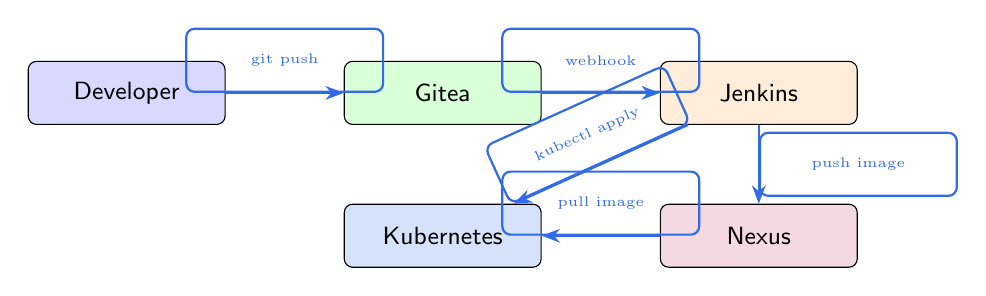
\begin{tikzpicture}[
  node distance=1cm and 1.5cm,
  every node/.style={rectangle,draw,rounded corners=3pt,minimum width=2.5cm,minimum height=0.8cm,font=\small\sffamily},
  arr/.style={->,>=Stealth,thick,k8sblue},
]
\node[fill=blue!15] (dev) {Developer};
\node[fill=green!15,right=of dev] (gitea) {Gitea};
\node[fill=orange!15,right=of gitea] (jenkins) {Jenkins};
\node[fill=purple!15,below=of jenkins] (nexus) {Nexus};
\node[fill=k8sblue!20,left=of nexus] (k8s) {Kubernetes};

\draw[arr] (dev) -- node[above,font=\tiny] {git push} (gitea);
\draw[arr] (gitea) -- node[above,font=\tiny] {webhook} (jenkins);
\draw[arr] (jenkins) -- node[right,font=\tiny] {push image} (nexus);
\draw[arr] (jenkins) -- node[above,font=\tiny,sloped] {kubectl apply} (k8s);
\draw[arr] (nexus) -- node[above,font=\tiny] {pull image} (k8s);
\end{tikzpicture}
\end{center}

\section{Gitea --- Self-hosted Git}

\begin{conceptbox}[Gitea]
\textbf{Chnoua:} Git server open-source, lightweight (Go). Alternative self-hosted l\'GitHub/GitLab.

\textbf{Fel projet mte3na:} Port 3000, deploy\'e b Docker Compose 3la services VM.

\textbf{Features:}
\begin{itemize}
  \item Git hosting (repos, branches, PRs)
  \item Issues + Wiki
  \item Webhooks (trigger Jenkins)
  \item CI/CD (Gitea Actions)
\end{itemize}
\end{conceptbox}

\textbf{URL:} \texttt{http://192.168.56.20:3000}

\section{Nexus --- Artifact Repository}

\begin{conceptbox}[Nexus Repository Manager]
\textbf{Chnoua:} Binary repository manager. Fi w\'ahid, yst\'okri 3\'ada types:
\begin{itemize}
  \item Docker images (registry)
  \item Maven JARs
  \item npm packages
  \item PyPI
  \item Raw files
\end{itemize}

\textbf{Fel projet mte3na:}
\begin{itemize}
  \item Port 8081: Nexus UI
  \item Port 8082: Docker registry endpoint
\end{itemize}
\end{conceptbox}

\subsection{Docker Registry Setup}

\begin{enumerate}
  \item Login l\'Nexus UI (\texttt{http://192.168.56.20:8081}) m3a \texttt{admin} + password mel container.
  \item Cr\'eer \tuni{Docker hosted repository} (\texttt{docker-hosted}).
  \item Assign HTTP port 8082.
  \item Sur Docker hosts: \texttt{/etc/docker/daemon.json}:
  \begin{lstlisting}
{
  "insecure-registries": ["192.168.56.20:8082"]
}
  \end{lstlisting}
  \item Push image:
  \begin{lstlisting}
docker tag myapp:v1 192.168.56.20:8082/myapp:v1
docker login 192.168.56.20:8082
docker push 192.168.56.20:8082/myapp:v1
  \end{lstlisting}
\end{enumerate}

\section{Jenkins --- CI/CD}

\begin{conceptbox}[Jenkins]
\textbf{Chnoua:} Automation server. Pipelines (Groovy), plugins (2000+), community enorme.

\textbf{Fel projet mte3na:} Port 8080, initial password printed during provisioning.

\textbf{Alternatives plus modernes:}
\begin{itemize}
  \item \textbf{GitLab CI}: Integrated m3a GitLab.
  \item \textbf{GitHub Actions}: Integrated m3a GitHub.
  \item \textbf{ArgoCD}: GitOps lel Kubernetes (declarative).
  \item \textbf{Tekton}: Kubernetes-native pipelines.
\end{itemize}
\end{conceptbox}

\subsection{Plugins N\'ecessaires}

\begin{itemize}
  \item \textbf{Kubernetes plugin}: Run agents as pods.
  \item \textbf{Docker plugin}: Build + push images.
  \item \textbf{Git plugin}: Clone repos.
  \item \textbf{Credentials plugin}: Manage secrets.
  \item \textbf{Blue Ocean}: Modern UI.
\end{itemize}

\subsection{Pipeline Example}

\begin{lstlisting}[caption={Jenkinsfile complet}]
pipeline {
  agent any
  environment {
    REGISTRY = '192.168.56.20:8082'
    IMAGE    = 'myapp'
  }
  stages {
    stage('Checkout') {
      steps {
        git url: 'http://192.168.56.20:3000/user/myapp.git'
      }
    }
    stage('Build') {
      steps {
        sh "docker build -t ${REGISTRY}/${IMAGE}:${BUILD_NUMBER} ."
      }
    }
    stage('Push') {
      steps {
        withCredentials([usernamePassword(
          credentialsId: 'nexus-creds',
          usernameVariable: 'USER',
          passwordVariable: 'PASS')]) {
          sh "echo $PASS | docker login -u $USER --password-stdin ${REGISTRY}"
          sh "docker push ${REGISTRY}/${IMAGE}:${BUILD_NUMBER}"
        }
      }
    }
    stage('Deploy') {
      steps {
        sh """
          kubectl set image deployment/myapp \
            myapp=${REGISTRY}/${IMAGE}:${BUILD_NUMBER} \
            --record
        """
      }
    }
  }
}
\end{lstlisting}

\cleardoublepage

% =============================================================================
\chapter{Storage Solution --- NFS}

\section{NFS Server fel Projet Mte3na}

\begin{conceptbox}[NFS (Network File System)]
\textbf{Chnoua:} Protocol yallaw mount filesystem distant comme s'il \'etait local.

\textbf{3leh fel K8s:} \texttt{ReadWriteMany} --- multiple pods 3la different nodes ynajmou yaqrawa w yketbou 3la nafs el data.

\textbf{Fel projet mte3na:}
\begin{itemize}
  \item Services VM: \texttt{192.168.56.20}
  \item Export: \texttt{/srv/nfs/mysql-data}
  \item Allowed network: \texttt{192.168.56.0/24}
\end{itemize}
\end{conceptbox}

\section{Exemple: MySQL m3a NFS}

\begin{lstlisting}[language=yaml]
# PV
apiVersion: v1
kind: PersistentVolume
metadata:
  name: mysql-pv
spec:
  capacity:
    storage: 10Gi
  accessModes: [ReadWriteMany]
  nfs:
    server: 192.168.56.20
    path: /srv/nfs/mysql-data
---
# PVC
apiVersion: v1
kind: PersistentVolumeClaim
metadata:
  name: mysql-pvc
spec:
  accessModes: [ReadWriteMany]
  resources:
    requests:
      storage: 10Gi
---
# Deployment
apiVersion: apps/v1
kind: Deployment
metadata:
  name: mysql
spec:
  replicas: 1
  selector:
    matchLabels: {app: mysql}
  template:
    metadata:
      labels: {app: mysql}
    spec:
      containers:
      - name: mysql
        image: mysql:8.0
        env:
        - name: MYSQL_ROOT_PASSWORD
          valueFrom:
            secretKeyRef:
              name: mysql-secret
              key: root-password
        volumeMounts:
        - name: data
          mountPath: /var/lib/mysql
      volumes:
      - name: data
        persistentVolumeClaim:
          claimName: mysql-pvc
\end{lstlisting}

\section{Alternatives lel NFS}

\begin{longtable}{L{3cm}L{9cm}}
\toprule
\textbf{Solution} & \textbf{When to use} \\
\midrule
NFS & Simple, existing NFS, dev/small prod \\
Rook/Ceph & Distributed, production, self-hosted clouds \\
Longhorn (Rancher) & Cloud-native, lightweight, backup included \\
OpenEBS & Storage for stateful workloads \\
Cloud (EBS, PD, Azure Disk) & Managed clouds \\
\bottomrule
\end{longtable}

\cleardoublepage

% =============================================================================
% PART 3: PRACTICAL SKILLS
% =============================================================================
\part{Practical Skills}

\chapter{kubectl Mastery}

\tuni{kubectl = sayf el DevOps}. Ken t\'s\'il\'ha, t\'sil 70\% mel K8s.

\section{Essential Commands}

\begin{longtable}{L{3cm}L{9cm}}
\toprule
\textbf{Command} & \textbf{Description} \\
\midrule
\cmd{get} & List resources \\
\cmd{describe} & Detailed info + events \\
\cmd{logs} & Container logs \\
\cmd{exec} & Execute command inside container \\
\cmd{apply} & Create or update from YAML \\
\cmd{delete} & Remove resource \\
\cmd{scale} & Change replicas count \\
\cmd{rollout} & Manage deployments (status, history, undo) \\
\cmd{port-forward} & Forward local port to pod \\
\cmd{cp} & Copy files to/from container \\
\cmd{top} & Show resource usage (needs metrics-server) \\
\cmd{edit} & Edit resource in place (\$EDITOR) \\
\cmd{config} & Manage kubeconfig contexts \\
\bottomrule
\end{longtable}

\section{Flags Critiques}

\begin{longtable}{L{3.5cm}L{8.5cm}}
\toprule
\textbf{Flag} & \textbf{Description} \\
\midrule
\texttt{-n <ns>} & Namespace \\
\texttt{-A, --all-namespaces} & Kol el namespaces \\
\texttt{-o yaml} & Output YAML \\
\texttt{-o json} & Output JSON \\
\texttt{-o wide} & More columns (IP, node, age) \\
\texttt{-o jsonpath=\{...\}} & Extract field \\
\texttt{-l <selector>} & Label selector (\texttt{app=nginx}) \\
\texttt{-w} & Watch for changes \\
\texttt{-f <file>} & From file \\
\texttt{--dry-run=client} & Test without applying \\
\texttt{-{}-previous} & Previous container (crashes) \\
\bottomrule
\end{longtable}

\section{Power Commands}

\begin{lstlisting}[caption={Commands kol DevOps lezmou y\'3rafhom}]
# Pod IPs + nodes
kubectl get pods -o wide

# Events (m\'ertabin bel time)
kubectl get events --sort-by=.metadata.creationTimestamp

# Resource usage
kubectl top nodes
kubectl top pods -A

# Delete pod (Deployment y3awd\'ou)
kubectl delete pod my-nginx-abc123

# Restart deployment (ma fammach restart mais...)
kubectl rollout restart deployment/my-nginx

# Port-forward (access service locally)
kubectl port-forward svc/my-service 8080:80

# Copy files
kubectl cp my-pod:/var/log/app.log ./app.log

# Exec interactive shell
kubectl exec -it my-pod -- /bin/bash

# Debug: ephemeral container (K8s 1.25+)
kubectl debug my-pod -it --image=busybox

# Generate YAML without applying
kubectl create deployment nginx --image=nginx --dry-run=client -o yaml

# Apply + save config
kubectl apply -f manifest.yaml --record

# Diff avant apply
kubectl diff -f manifest.yaml
\end{lstlisting}

\section{kubectl Aliases (Productivity)}

\begin{lstlisting}[caption={Zid fi .bashrc / .zshrc}]
alias k='kubectl'
alias kgp='kubectl get pods'
alias kgs='kubectl get services'
alias kgd='kubectl get deployments'
alias kaf='kubectl apply -f'
alias kdel='kubectl delete'
alias klog='kubectl logs'
alias kexec='kubectl exec -it'
alias kctx='kubectl config current-context'
alias kns='kubectl config set-context --current --namespace'

# Enable autocompletion
source <(kubectl completion bash)
complete -F __start_kubectl k
\end{lstlisting}

\section{Debugging Techniques}

\subsection{Pod Stuck en Pending}

\begin{lstlisting}
kubectl describe pod <name>
# Lawej fi "Events" section:
#  - Insufficient cpu/memory → node ma y\'k\'afich
#  - No nodes available → nodeSelector/taints problem
#  - FailedScheduling → ressources k'afr\'ikin
\end{lstlisting}

\subsection{CrashLoopBackOff}

\begin{lstlisting}
# Logs mel container el akher crashi
kubectl logs <pod> --previous

# Check exit code
kubectl describe pod <pod>

# Common causes:
# - Config manquante
# - Liveness probe yet\'en5as
# - Missing dependency (DB down)
# - Application bug
\end{lstlisting}

\subsection{ImagePullBackOff}

\begin{lstlisting}
kubectl describe pod <pod>
# Events:
# - "manifest unknown" → image tag incorrect
# - "unauthorized" → lezem imagePullSecret
# - "no such host" → network / DNS problem
\end{lstlisting}

\cleardoublepage

% =============================================================================
\chapter{YAML Manifests Mastery}

\section{Structure Standard}

\begin{lstlisting}[language=yaml]
apiVersion: <group/version>   # e.g., apps/v1, v1, networking.k8s.io/v1
kind: <ResourceType>          # Pod, Deployment, Service, etc.
metadata:
  name: <name>                # Unique per namespace
  namespace: <ns>             # Optional, default "default"
  labels:                     # Key-value pairs for selection
    key: value
  annotations:                # Key-value pairs for metadata
    key: value
spec:
  # Resource-specific configuration
\end{lstlisting}

\section{Best Practices}

\begin{enumerate}
  \item \textbf{Toujours est3mel Deployment, mouch Pod tout seul.}
  \item \textbf{Define resource requests + limits.} Sans, scheduling random, evictions surprises.
  \item \textbf{Use labels consistently.} \texttt{app}, \texttt{version}, \texttt{env}, \texttt{tier}.
  \item \textbf{Separate configs m3a ConfigMap + Secret.} Ma t\'hard\'c\'odi.
  \item \textbf{Readiness + Liveness probes.} Essentials for zero-downtime deploys.
  \item \textbf{Use namespaces.} Separate environments, teams.
  \item \textbf{Version your manifests.} Git repo, review via PRs (GitOps).
  \item \textbf{Use Helm wla Kustomize.} Ma tcopierch nafs manifest 10 marra.
\end{enumerate}

\section{Probes --- Health Checks}

\begin{lstlisting}[language=yaml]
containers:
- name: app
  image: myapp:v1
  livenessProbe:           # Ken yeche, restart container
    httpGet:
      path: /healthz
      port: 8080
    initialDelaySeconds: 30
    periodSeconds: 10
  readinessProbe:          # Ken yeche, ra7el mel service endpoints
    httpGet:
      path: /ready
      port: 8080
    initialDelaySeconds: 5
    periodSeconds: 5
  startupProbe:            # Lel apps qui 5adhen wa9t tebdet
    httpGet:
      path: /startup
      port: 8080
    failureThreshold: 30
    periodSeconds: 10
\end{lstlisting}

\begin{tipbox}
\textbf{Rule of thumb lel probes:}
\begin{itemize}
  \item \texttt{startupProbe}: lel slow-start apps (JVMs, Rails).
  \item \texttt{readinessProbe}: Check ken ready yakoul traffic.
  \item \texttt{livenessProbe}: Check ken mazal alive (ken dead → restart).
\end{itemize}
\textbf{Ma t5attich livenessProbe aggressive} ken app mte3ek slow-start!
\end{tipbox}

\cleardoublepage

% =============================================================================
\chapter{Troubleshooting Guide}

\section{Node Issues}

\subsection{Node NotReady}

\begin{lstlisting}
# Step 1: Status
kubectl get nodes
kubectl describe node <name>

# Step 2: kubelet 3al node
vagrant ssh <node>
sudo systemctl status kubelet
sudo journalctl -u kubelet -f

# Common causes:
# - kubelet qaf\'ech → restart
# - containerd down → sudo systemctl restart containerd
# - Disk pressure → df -h, clean images
# - Memory pressure → check workloads
# - Network: can't reach API server → check routing
\end{lstlisting}

\subsection{Disk Pressure}

\begin{lstlisting}
# Check disk
df -h

# Clean unused images (3al node)
sudo crictl rmi --prune

# Clean pod logs
sudo find /var/log/pods -type f -size +100M
\end{lstlisting}

\section{Pod Issues}

\subsection{Decision Tree}

\begin{center}
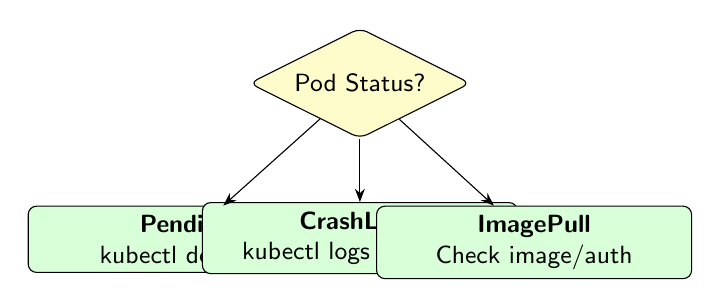
\begin{tikzpicture}[
  node distance=0.8cm,
  every node/.style={rectangle,draw,rounded corners=3pt,font=\small\sffamily,align=center},
  decision/.style={diamond,aspect=2,fill=yellow!20},
  action/.style={fill=green!15,minimum width=4cm},
  arr/.style={->,>=Stealth},
]
\node[decision] (d1) {Pod Status?};
\node[action,below left=1.2cm and -0.5cm of d1] (pending) {\textbf{Pending}\\kubectl describe};
\node[action,below=of d1] (crash) {\textbf{CrashLoop}\\kubectl logs --previous};
\node[action,below right=1.2cm and -0.5cm of d1] (imgpull) {\textbf{ImagePull}\\Check image/auth};

\draw[arr] (d1) -- (pending);
\draw[arr] (d1) -- (crash);
\draw[arr] (d1) -- (imgpull);
\end{tikzpicture}
\end{center}

\section{Network Issues}

\subsection{DNS Ma Y5adchi}

\begin{lstlisting}
# Test dns mel pod
kubectl run -it --rm debug --image=busybox --restart=Never -- sh
/ # nslookup kubernetes
/ # nslookup my-service.default

# Check coredns pods
kubectl get pods -n kube-system -l k8s-app=kube-dns
kubectl logs -n kube-system -l k8s-app=kube-dns
\end{lstlisting}

\subsection{Service Ma Yo7ouzch Traffic}

\begin{lstlisting}
# Check endpoints (pods match\'es bel selector)
kubectl get endpoints my-service
# Ken vide → selector yenfa ala pods

# Check pods labels
kubectl get pods --show-labels

# Test mel pod debug
kubectl run -it --rm debug --image=nicolaka/netshoot --restart=Never -- \
  curl http://my-service.default.svc.cluster.local
\end{lstlisting}

\subsection{Cross-node Communication (CNI)}

\begin{lstlisting}
# Flannel pods healthy?
kubectl get pods -n kube-flannel

# Logs
kubectl logs -n kube-flannel -l app=flannel

# Test pod-to-pod cross node
# Pod A on node1 → ping Pod B on node2 IP
\end{lstlisting}

\section{Cluster-Wide Debugging}

\begin{lstlisting}
# Health of control plane
kubectl get pods -n kube-system
kubectl get componentstatuses  # deprecated b K8s 1.19+

# Cluster info
kubectl cluster-info
kubectl cluster-info dump > cluster-debug.log

# Events globaux (toujours critical!)
kubectl get events -A --sort-by=.metadata.creationTimestamp | tail -30
\end{lstlisting}

\cleardoublepage

% =============================================================================
\chapter{Production Readiness}

\section{High Availability}

\subsection{Control Plane HA}

\begin{itemize}
  \item \textbf{3 (or 5) master nodes.} Odd numbers (quorum).
  \item \textbf{External etcd cluster} wla \textbf{stacked etcd}.
  \item \textbf{Load balancer} lel API server (HAProxy, keepalived, cloud LB).
\end{itemize}

\subsection{Application HA}

\begin{itemize}
  \item \texttt{replicas >= 2}
  \item \texttt{PodDisruptionBudget} (ma ta7atch all pods down at once)
  \item \texttt{topologySpreadConstraints} (spread across zones/nodes)
\end{itemize}

\begin{lstlisting}[language=yaml,caption={PodDisruptionBudget}]
apiVersion: policy/v1
kind: PodDisruptionBudget
metadata:
  name: my-app-pdb
spec:
  minAvailable: 2
  selector:
    matchLabels:
      app: my-app
\end{lstlisting}

\section{Backup \& Disaster Recovery}

\subsection{etcd Snapshots}

\begin{lstlisting}
# Manual snapshot
sudo ETCDCTL_API=3 etcdctl \
  --endpoints=https://127.0.0.1:2379 \
  --cacert=/etc/kubernetes/pki/etcd/ca.crt \
  --cert=/etc/kubernetes/pki/etcd/server.crt \
  --key=/etc/kubernetes/pki/etcd/server.key \
  snapshot save /backup/etcd-$(date +%F).db
\end{lstlisting}

Automate via CronJob, backup l\'S3/NFS.

\subsection{Velero --- Cluster Backup}

\begin{conceptbox}[Velero]
\textbf{Chnoua:} Backup + restore tool lel Kubernetes clusters. Backup PVs (b snapshots) + resources (YAML).

\textbf{Use cases:} Migration, DR, schedule backups.
\end{conceptbox}

\subsection{GitOps --- Declarative Recovery}

Ken kol manifests fel Git, tnajem ta3mel cluster jdid + \cmd{kubectl apply -f} = restore. Tools: \tech{ArgoCD}, \tech{Flux}.

\section{Security Hardening}

\begin{itemize}
  \item \textbf{RBAC enabled} (default b kubeadm).
  \item \textbf{Network Policies} (default deny + explicit allow).
  \item \textbf{Pod Security Standards} (restricted profile).
  \item \textbf{Secrets encryption at rest} (etcd).
  \item \textbf{TLS everywhere} (API server, etcd, kubelet).
  \item \textbf{Regular updates} (CVEs patchouhom f\'essa3).
  \item \textbf{Image scanning} (Trivy, Clair, Grype).
  \item \textbf{Admission controllers} (OPA Gatekeeper, Kyverno).
\end{itemize}

\section{Monitoring \& Alerting}

\textbf{Stack minimum viable:}
\begin{itemize}
  \item Prometheus (metrics)
  \item Grafana (dashboards)
  \item Alertmanager (alerts)
  \item Loki (logs)
  \item kube-state-metrics (cluster metrics)
  \item node-exporter (node metrics)
\end{itemize}

\textbf{Alerts critiques:}
\begin{itemize}
  \item Node NotReady > 5 min
  \item Pod restart rate > 5/hour
  \item API server latency > 1s
  \item etcd disk full > 80\%
  \item Certificate expiration < 30 days
\end{itemize}

\cleardoublepage

% =============================================================================
% PART 4: NEXT STEPS
% =============================================================================
\part{Next Steps}

\chapter{Learning Path}

\section{Roadmap lel 6 Mois}

\begin{enumerate}
  \item \textbf{Semaine 1-2:} Master kubectl, YAML manifests (hedha ktib).
  \item \textbf{Semaine 3-4:} Deploy real applications (nginx, WordPress, MySQL).
  \item \textbf{Mois 2:} Helm (package manager).
  \item \textbf{Mois 2-3:} CI/CD m3a Jenkins/GitLab/ArgoCD.
  \item \textbf{Mois 3-4:} Monitoring stack (Prometheus + Grafana).
  \item \textbf{Mois 4-5:} Security (RBAC, Network Policies, OPA).
  \item \textbf{Mois 5-6:} Cloud K8s (EKS/GKE) + service mesh (Istio).
\end{enumerate}

\section{Certifications}

\begin{longtable}{L{3cm}L{4cm}L{5cm}}
\toprule
\textbf{Cert} & \textbf{Level} & \textbf{Focus} \\
\midrule
CKAD & Developer & Apps, deployments, services \\
CKA & Admin & Cluster mgmt, networking, storage \\
CKS & Security & Hardening, RBAC, policies \\
\bottomrule
\end{longtable}

\textbf{Tips:}
\begin{itemize}
  \item Practice 3la \href{https://killer.sh}{killer.sh} (simulator officiel).
  \item Timing est key --- 2 heures lel 17-20 questions.
  \item \cmd{alias k=kubectl} mal awal 7aja!
\end{itemize}

\cleardoublepage

% =============================================================================
\chapter{Hands-on Exercises}

Lou ken t\'es\'l\'i7t ktib heda lelk\'olou, essai les exercices hedhom 3al cluster mte3ek:

\section{Level 1: Basics}

\begin{enumerate}
  \item Deploy nginx b 3 replicas.
  \item Expose via NodePort service.
  \item Access mel browser 3al \texttt{http://192.168.56.10:<nodeport>}.
  \item Scale l\'5 replicas.
  \item Watch pods (\cmd{kubectl get pods -w}) w delete pod we7ed --- observe comment K8s recreate.
\end{enumerate}

\section{Level 2: Intermediate}

\begin{enumerate}
  \item Rolling update: nginx:1.25 → nginx:1.26 b zero downtime.
  \item Rollback awel version.
  \item Create ConfigMap + inject as env vars.
  \item Create Secret (base64) + mount as file.
  \item Add persistent volume m3a NFS.
  \item Resource requests + limits + observe scheduling.
\end{enumerate}

\section{Level 3: Advanced}

\begin{enumerate}
  \item Deploy multi-tier app (frontend + backend + MySQL).
  \item Configure liveness + readiness probes.
  \item Setup Ingress controller (nginx-ingress).
  \item Install Helm + deploy WordPress via chart.
  \item Install Prometheus + Grafana (kube-prometheus-stack).
  \item Write CronJob l\'database backup dawri.
\end{enumerate}

\section{Level 4: Expert}

\begin{enumerate}
  \item Setup CI/CD: Gitea push → Jenkins build → Nexus push → kubectl apply.
  \item Implement NetworkPolicies (switch l\'Calico).
  \item Enable Pod Security Standards.
  \item Setup ArgoCD + GitOps workflow.
  \item Deploy Istio service mesh.
  \item Disaster recovery: backup etcd, destroy cluster, restore.
\end{enumerate}

\cleardoublepage

% =============================================================================
\chapter{Resources}

\section{Official}

\begin{itemize}
  \item \href{https://kubernetes.io/docs/}{kubernetes.io/docs} --- \tuni{Bible officielle}.
  \item \href{https://kubernetes.io/docs/reference/kubectl/cheatsheet/}{kubectl Cheatsheet}.
  \item \href{https://landscape.cncf.io}{CNCF Landscape} --- Chouf ecosystem kolou.
\end{itemize}

\section{Books}

\begin{itemize}
  \item \textit{Kubernetes in Action} --- Marko Lukša (\tuni{classic}).
  \item \textit{Kubernetes Up \& Running} --- Hightower, Burns, Beda.
  \item \textit{Kubernetes Patterns} --- Ibryam, Huss.
  \item \textit{Programming Kubernetes} --- Hausenblas (pour Operators).
\end{itemize}

\section{Free Learning}

\begin{itemize}
  \item \href{https://github.com/kelseyhightower/kubernetes-the-hard-way}{Kubernetes the Hard Way} --- Kelsey Hightower.
  \item \href{https://www.katacoda.com}{Katacoda} (archived but useful).
  \item \href{https://killercoda.com}{Killercoda} (interactive scenarios).
  \item \href{https://labs.play-with-k8s.com}{Play with Kubernetes}.
\end{itemize}

\section{Communities}

\begin{itemize}
  \item \href{https://slack.k8s.io}{Kubernetes Slack} (70k+ members).
  \item \href{https://www.reddit.com/r/kubernetes}{r/kubernetes}.
  \item \href{https://discuss.kubernetes.io}{discuss.kubernetes.io}.
\end{itemize}

\section{Tools t\'ksebha}

\begin{itemize}
  \item \tech{k9s} --- Terminal UI pour K8s (\tuni{yfou9ek klal}).
  \item \tech{stern} --- Multi-pod log tailing.
  \item \tech{kubectx} + \tech{kubens} --- Switch contexts/namespaces f\'essa3.
  \item \tech{lens} --- GUI pour K8s.
  \item \tech{kubeseal} --- Sealed Secrets CLI.
  \item \tech{helm} --- Package manager.
  \item \tech{skaffold} --- Dev workflow.
  \item \tech{kustomize} --- Config management (built into kubectl).
\end{itemize}

% =============================================================================
\chapter*{Conclusion}
\addcontentsline{toc}{chapter}{Conclusion}

\tuni{Ya sa7bi}, ken wselt el ghaya mel ktib heda, \tuni{chapo!} Mush k\'ol 7ad yfout fi 150+ page mta3 Kubernetes.

El 7a9i9a: \textbf{learning Kubernetes mouch destination, houa voyage.} Ecosystem yetwalled kol j\'oum. Operators jdod, CNIs jdud, patterns jdud.

\textbf{Maz\'eit:}
\begin{enumerate}
  \item \tuni{Efhem avant ma t7fdh.} Concepts > commands.
  \item \tuni{Pratique kol y\'oum.} Deploy 7aja, 7atta ken nginx.
  \item \tuni{Rea\`d post-mortems.} Ki cluster y5asser 3\'and 5arr\'nn\'in, efhem el root cause.
  \item \tuni{Join community.} Slack, Reddit, meetups.
  \item \tuni{Contribuer.} Documentation, bug reports, meme ken 7aja 9\'asira.
\end{enumerate}

\textbf{Rappel:}
\begin{center}
\Large\itshape
\emph{"In production, complexity is the enemy."}\\
\normalfont\normalsize --- Kelsey Hightower
\end{center}

K\'olma t\'si kubernetes deployment complex, rod roye\'k. Fih solution m basset?

Success fi rihletek! 🚀

\vspace{1cm}
\begin{center}
\textbf{--- El Ktib Kemel ---}\\[0.3cm]
\small\textit{Lou ken sebit fi errors wla 7abb t\'zid 7ajjat, open PR 3al repo.}
\end{center}

\end{document}
